\documentclass[a4paper]{book}
\usepackage{makeidx}
\usepackage{graphicx}
\usepackage{multicol}
\usepackage{float}
\usepackage{listings}
\usepackage{color}
\usepackage{ifthen}
\usepackage[table]{xcolor}
\usepackage{textcomp}
\usepackage{alltt}
\usepackage{ifpdf}
\ifpdf
\usepackage[pdftex,
            pagebackref=true,
            colorlinks=true,
            linkcolor=blue,
            unicode
           ]{hyperref}
\else
\usepackage[ps2pdf,
            pagebackref=true,
            colorlinks=true,
            linkcolor=blue,
            unicode
           ]{hyperref}
\usepackage{pspicture}
\fi
\usepackage[utf8]{inputenc}
\usepackage[brazil]{babel}
\usepackage{mathptmx}
\usepackage[scaled=.90]{helvet}
\usepackage{courier}
\usepackage{sectsty}
\usepackage[titles]{tocloft}
\usepackage{doxygen}
\lstset{language=C++,inputencoding=utf8,basicstyle=\footnotesize,breaklines=true,breakatwhitespace=true,tabsize=8,numbers=left }
\makeindex
\setcounter{tocdepth}{3}
\renewcommand{\footrulewidth}{0.4pt}
\renewcommand{\familydefault}{\sfdefault}
\begin{document}
\hypersetup{pageanchor=false}
\begin{titlepage}
\vspace*{7cm}
\begin{center}
{\Large Gunther's Quest Alpha \\[1ex]\large 0.2 }\\
\vspace*{1cm}
{\large Gerado por Doxygen 1.7.4}\\
\vspace*{0.5cm}
{\small Terça, 17 de Julho de 2012 22:45:47}\\
\end{center}
\end{titlepage}
\clearemptydoublepage
\pagenumbering{roman}
\tableofcontents
\clearemptydoublepage
\pagenumbering{arabic}
\hypersetup{pageanchor=true}
\chapter{Índice das Estruturas de Dados}
\section{Estruturas de Dados}
Aqui estão as estruturas de dados, uniões e suas respectivas descrições\-:\begin{DoxyCompactList}
\item\contentsline{section}{\hyperlink{struct__jogador}{\-\_\-jogador} }{\pageref{struct__jogador}}{}
\item\contentsline{section}{\hyperlink{struct__ladrilho}{\-\_\-ladrilho} }{\pageref{struct__ladrilho}}{}
\item\contentsline{section}{\hyperlink{struct__objeto}{\-\_\-objeto} }{\pageref{struct__objeto}}{}
\item\contentsline{section}{\hyperlink{struct__tabuleiro}{\-\_\-tabuleiro} }{\pageref{struct__tabuleiro}}{}
\item\contentsline{section}{\hyperlink{structstruct__objeto}{struct\-\_\-objeto} }{\pageref{structstruct__objeto}}{}
\item\contentsline{section}{\hyperlink{structstruct__vetor}{struct\-\_\-vetor} }{\pageref{structstruct__vetor}}{}
\end{DoxyCompactList}

\chapter{Índice dos Arquivos}
\section{Lista de Arquivos}
Esta é a lista de todos os arquivos documentados e suas respectivas descrições\-:\begin{DoxyCompactList}
\item\contentsline{section}{include/\hyperlink{gunther_8h}{gunther.\-h} \\*Arquivo header geral do jogo }{\pageref{gunther_8h}}{}
\item\contentsline{section}{include/\hyperlink{rkefisica_8h}{rkefisica.\-h} \\*Arquivo header da biblioteca de funções físicas }{\pageref{rkefisica_8h}}{}
\item\contentsline{section}{include/\hyperlink{rkegraficos_8h}{rkegraficos.\-h} \\*Arquivo header da parte gráfica }{\pageref{rkegraficos_8h}}{}
\item\contentsline{section}{include/\hyperlink{rkerender_8h}{rkerender.\-h} \\*Arquivo header do renderizador }{\pageref{rkerender_8h}}{}
\item\contentsline{section}{include/\hyperlink{rketypes_8h}{rketypes.\-h} \\*Arquivo header de tipos e defines do Red Knife Engine }{\pageref{rketypes_8h}}{}
\item\contentsline{section}{src/\hyperlink{main_8c}{main.\-c} \\*Ponto de entrada do jogo }{\pageref{main_8c}}{}
\item\contentsline{section}{src/menu/\hyperlink{menu_8c}{menu.\-c} \\*Implementação do menu principal }{\pageref{menu_8c}}{}
\item\contentsline{section}{src/rkegraficos/\hyperlink{rkegraficos_8c}{rkegraficos.\-c} \\*Utilitários gráficos }{\pageref{rkegraficos_8c}}{}
\item\contentsline{section}{src/rkerender/\hyperlink{rkerender_8c}{rkerender.\-c} \\*Renderizador de fases }{\pageref{rkerender_8c}}{}
\end{DoxyCompactList}

\chapter{Estruturas}
\hypertarget{struct__jogador}{
\section{Referência da Estrutura \_\-jogador}
\label{struct__jogador}\index{\_\-jogador@{\_\-jogador}}
}


{\ttfamily \#include $<$player.h$>$}

\subsection*{Campos de Dados}
\begin{DoxyCompactItemize}
\item 
\hypertarget{struct__jogador_a10a4d4bb1fa867a1c3a9bc2ab9ee7e9d}{
SDL\_\-Rect {\bfseries retangulo} \mbox{[}8\mbox{]}}
\label{struct__jogador_a10a4d4bb1fa867a1c3a9bc2ab9ee7e9d}

\item 
\hypertarget{struct__jogador_a6150e0515f7202e2fb518f7206ed97dc}{
int {\bfseries x}}
\label{struct__jogador_a6150e0515f7202e2fb518f7206ed97dc}

\item 
\hypertarget{struct__jogador_a0a2f84ed7838f07779ae24c5a9086d33}{
int {\bfseries y}}
\label{struct__jogador_a0a2f84ed7838f07779ae24c5a9086d33}

\item 
\hypertarget{struct__jogador_a05818f82142eb45301bf89e8939bb8ae}{
int {\bfseries direcao}}
\label{struct__jogador_a05818f82142eb45301bf89e8939bb8ae}

\item 
\hypertarget{struct__jogador_a9aa790f93d2d067a4f5608fdb8409f94}{
int {\bfseries hp}}
\label{struct__jogador_a9aa790f93d2d067a4f5608fdb8409f94}

\item 
\hypertarget{struct__jogador_a5819a445ff2fb05f613477829c04f115}{
int {\bfseries poder\_\-flecha}}
\label{struct__jogador_a5819a445ff2fb05f613477829c04f115}

\item 
\hypertarget{struct__jogador_a7ba2606514453e5bedf98b5510b8169e}{
int {\bfseries poder\_\-bomba}}
\label{struct__jogador_a7ba2606514453e5bedf98b5510b8169e}

\item 
\hypertarget{struct__jogador_a06e0ae6abeebe6c53b256cca1e00fedf}{
int {\bfseries bombas}}
\label{struct__jogador_a06e0ae6abeebe6c53b256cca1e00fedf}

\end{DoxyCompactItemize}


\subsection{Descrição Detalhada}
Struct Jogador 
\begin{DoxyParams}{Parâmetros}
{\em retangulo} & Vetor com os 8 retângulos das visões do jogador \\
\hline
{\em x} & Posição x do jogador \\
\hline
{\em y} & Posição y do jogador \\
\hline
{\em direcao} & Direção que o jogador está olhando \\
\hline
{\em hp} & Quantidade de hp do jogador \\
\hline
\end{DoxyParams}


A documentação para esta estrutura foi gerada a partir do seguinte arquivo:\begin{DoxyCompactItemize}
\item 
\hyperlink{player_8h}{player.h}\end{DoxyCompactItemize}

\hypertarget{structatt}{
\section{Referência da Estrutura att}
\label{structatt}\index{att@{att}}
}
\subsection*{Campos de Dados}
\begin{DoxyCompactItemize}
\item 
\hypertarget{structatt_afddb4eaa163c31ce59f5e1f6f47650f4}{
attackType {\bfseries type}}
\label{structatt_afddb4eaa163c31ce59f5e1f6f47650f4}

\item 
\hypertarget{structatt_a037e8e370380046bec287bdc96942091}{
int {\bfseries range}}
\label{structatt_a037e8e370380046bec287bdc96942091}

\item 
\hypertarget{structatt_a7b53939b690d58264414abe55f6b156b}{
int {\bfseries firerate}}
\label{structatt_a7b53939b690d58264414abe55f6b156b}

\item 
\hypertarget{structatt_a9b39867abc3f09243fcdc739bd9e6c90}{
int {\bfseries damage}}
\label{structatt_a9b39867abc3f09243fcdc739bd9e6c90}

\end{DoxyCompactItemize}


A documentação para esta estrutura foi gerada a partir do seguinte arquivo:\begin{DoxyCompactItemize}
\item 
\hyperlink{game_8h}{game.h}\end{DoxyCompactItemize}

\hypertarget{structgmboard}{
\section{Referência da Estrutura gmboard}
\label{structgmboard}\index{gmboard@{gmboard}}
}


Diagrama de colaboração para gmboard:\nopagebreak
\begin{figure}[H]
\begin{center}
\leavevmode
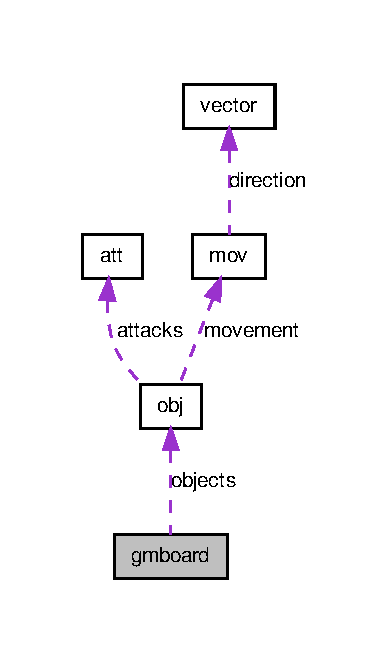
\includegraphics[width=187pt]{structgmboard__coll__graph}
\end{center}
\end{figure}
\subsection*{Campos de Dados}
\begin{DoxyCompactItemize}
\item 
\hypertarget{structgmboard_ac93f4d34cf045e33f4ef3b0852758a6f}{
char {\bfseries scenario} \mbox{[}BOARD\_\-HEIGHT\mbox{]}\mbox{[}BOARD\_\-WIDTH\mbox{]}}
\label{structgmboard_ac93f4d34cf045e33f4ef3b0852758a6f}

\item 
\hypertarget{structgmboard_a329a8c751b484ac4562b5334174cd9b5}{
\hyperlink{structobj}{Object} $\ast$ {\bfseries objects} \mbox{[}BOARD\_\-HEIGHT\mbox{]}\mbox{[}BOARD\_\-WIDTH\mbox{]}}
\label{structgmboard_a329a8c751b484ac4562b5334174cd9b5}

\end{DoxyCompactItemize}


A documentação para esta estrutura foi gerada a partir do seguinte arquivo:\begin{DoxyCompactItemize}
\item 
\hyperlink{game_8h}{game.h}\end{DoxyCompactItemize}

\hypertarget{structmov}{
\section{Referência da Estrutura mov}
\label{structmov}\index{mov@{mov}}
}


Diagrama de colaboração para mov:\nopagebreak
\begin{figure}[H]
\begin{center}
\leavevmode
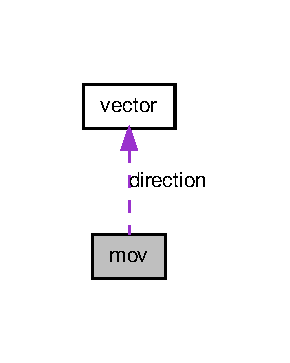
\includegraphics[width=139pt]{structmov__coll__graph}
\end{center}
\end{figure}
\subsection*{Campos de Dados}
\begin{DoxyCompactItemize}
\item 
\hypertarget{structmov_aecb8547c3f519debb1e12fcf4629d05c}{
movementPattern {\bfseries pattern}}
\label{structmov_aecb8547c3f519debb1e12fcf4629d05c}

\item 
\hypertarget{structmov_a218b4f7c6cc2681a99c23a3b089d68b1}{
int {\bfseries speed}}
\label{structmov_a218b4f7c6cc2681a99c23a3b089d68b1}

\item 
\hypertarget{structmov_a2db09f9fefd93b32aad2f340ad270622}{
\hyperlink{structvector}{Vector} {\bfseries direction}}
\label{structmov_a2db09f9fefd93b32aad2f340ad270622}

\item 
\hypertarget{structmov_a2f16194304829daa3f050ba49f218b5f}{
int {\bfseries expire}}
\label{structmov_a2f16194304829daa3f050ba49f218b5f}

\end{DoxyCompactItemize}


A documentação para esta estrutura foi gerada a partir do seguinte arquivo:\begin{DoxyCompactItemize}
\item 
\hyperlink{game_8h}{game.h}\end{DoxyCompactItemize}

\hypertarget{structobj}{
\section{Referência da Estrutura obj}
\label{structobj}\index{obj@{obj}}
}


Diagrama de colaboração para obj:\nopagebreak
\begin{figure}[H]
\begin{center}
\leavevmode
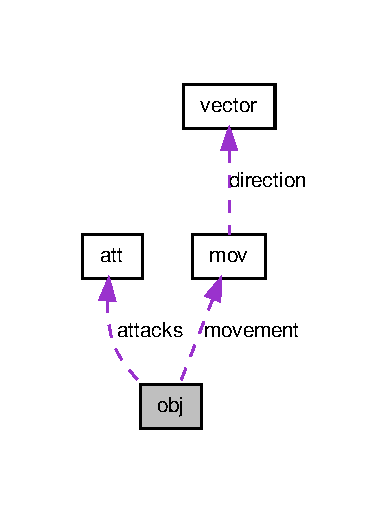
\includegraphics[width=187pt]{structobj__coll__graph}
\end{center}
\end{figure}
\subsection*{Campos de Dados}
\begin{DoxyCompactItemize}
\item 
\hypertarget{structobj_a86d156fc82d183ec8f4967283abea2fa}{
char {\bfseries name} \mbox{[}MAXLEN\mbox{]}}
\label{structobj_a86d156fc82d183ec8f4967283abea2fa}

\item 
\hypertarget{structobj_af749ccd9c242573390416d80accd7b39}{
char {\bfseries id}}
\label{structobj_af749ccd9c242573390416d80accd7b39}

\item 
\hypertarget{structobj_a58ca25ca6c9448a364b84539e42f1fa6}{
int {\bfseries HP}}
\label{structobj_a58ca25ca6c9448a364b84539e42f1fa6}

\item 
\hypertarget{structobj_a2f16194304829daa3f050ba49f218b5f}{
int {\bfseries expire}}
\label{structobj_a2f16194304829daa3f050ba49f218b5f}

\item 
\hypertarget{structobj_ac6c1517a5d26b836cf93f7dd26c0269d}{
bool {\bfseries attackOthers}}
\label{structobj_ac6c1517a5d26b836cf93f7dd26c0269d}

\item 
\hypertarget{structobj_af45a8a8dc17b18be6e6a4d951424c4c9}{
\hyperlink{structmov}{Movement} {\bfseries movement}}
\label{structobj_af45a8a8dc17b18be6e6a4d951424c4c9}

\item 
\hypertarget{structobj_a8130237828c5c7edea161ac2642d5b31}{
int {\bfseries numAttacks}}
\label{structobj_a8130237828c5c7edea161ac2642d5b31}

\item 
\hypertarget{structobj_acde888f5f7e2f77fb48eaca6cf2a6dc3}{
\hyperlink{structatt}{Attack} {\bfseries attacks} \mbox{[}MAXATTACKS\mbox{]}}
\label{structobj_acde888f5f7e2f77fb48eaca6cf2a6dc3}

\item 
\hypertarget{structobj_ae3a34d17b75971c48ca48550c1d95b90}{
int {\bfseries numImmunities}}
\label{structobj_ae3a34d17b75971c48ca48550c1d95b90}

\item 
\hypertarget{structobj_a2c4d35a751f31c8e4f8febdc8b141f69}{
attackType {\bfseries immunities} \mbox{[}MAXIMMUNITIES\mbox{]}}
\label{structobj_a2c4d35a751f31c8e4f8febdc8b141f69}

\item 
\hypertarget{structobj_aec06a54fb1cc6faf5a3d3e2232572cc5}{
SDL\_\-Rect {\bfseries clip}}
\label{structobj_aec06a54fb1cc6faf5a3d3e2232572cc5}

\end{DoxyCompactItemize}


A documentação para esta estrutura foi gerada a partir do seguinte arquivo:\begin{DoxyCompactItemize}
\item 
\hyperlink{game_8h}{game.h}\end{DoxyCompactItemize}

\hypertarget{structterreno}{
\section{Referência da Estrutura terreno}
\label{structterreno}\index{terreno@{terreno}}
}
\subsection*{Campos de Dados}
\begin{DoxyCompactItemize}
\item 
\hypertarget{structterreno_af4541a0087b5e63cdca818a994d5119c}{
int {\bfseries passavel}}
\label{structterreno_af4541a0087b5e63cdca818a994d5119c}

\item 
\hypertarget{structterreno_a66706353d918fc22d4b7130ef5a9fbc4}{
SDL\_\-Rect {\bfseries retangulo}}
\label{structterreno_a66706353d918fc22d4b7130ef5a9fbc4}

\end{DoxyCompactItemize}


A documentação para esta estrutura foi gerada a partir do seguinte arquivo:\begin{DoxyCompactItemize}
\item 
\hyperlink{game_8h}{game.h}\end{DoxyCompactItemize}

\hypertarget{structvector}{
\section{Referência da Estrutura vector}
\label{structvector}\index{vector@{vector}}
}
\subsection*{Campos de Dados}
\begin{DoxyCompactItemize}
\item 
\hypertarget{structvector_a6150e0515f7202e2fb518f7206ed97dc}{
int {\bfseries x}}
\label{structvector_a6150e0515f7202e2fb518f7206ed97dc}

\item 
\hypertarget{structvector_a0a2f84ed7838f07779ae24c5a9086d33}{
int {\bfseries y}}
\label{structvector_a0a2f84ed7838f07779ae24c5a9086d33}

\end{DoxyCompactItemize}


A documentação para esta estrutura foi gerada a partir do seguinte arquivo:\begin{DoxyCompactItemize}
\item 
\hyperlink{game_8h}{game.h}\end{DoxyCompactItemize}

\chapter{Arquivos}
\hypertarget{boardloader_8c}{
\section{Referência do Arquivo boardloader.c}
\label{boardloader_8c}\index{boardloader.c@{boardloader.c}}
}


Funções para carregar as informações pertinentes a monstros, terrenos, objetos, fases a partir de seus arquivos de dados.  


{\ttfamily \#include \char`\"{}player.h\char`\"{}}\par
Gráfico de dependência de inclusões para boardloader.c:\nopagebreak
\begin{figure}[H]
\begin{center}
\leavevmode
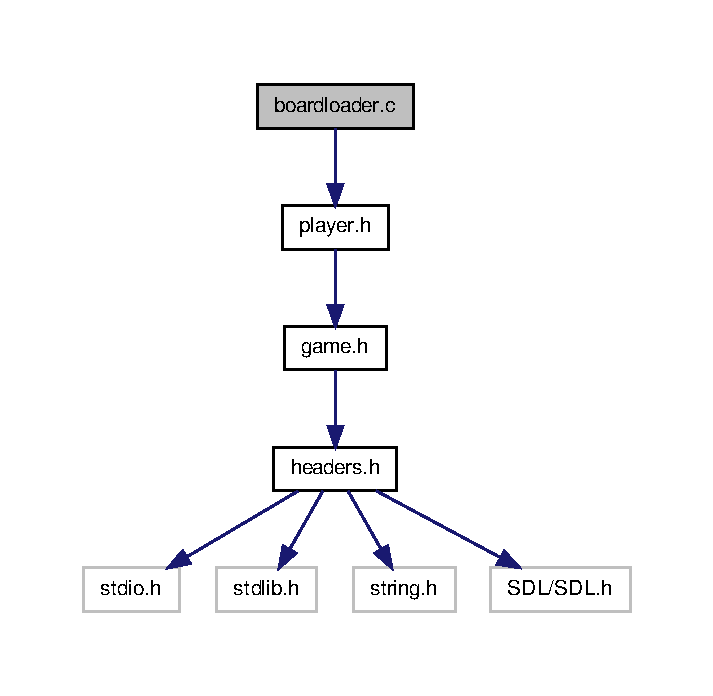
\includegraphics[width=342pt]{boardloader_8c__incl}
\end{center}
\end{figure}
\subsection*{Funções}
\begin{DoxyCompactItemize}
\item 
void \hyperlink{boardloader_8c_afc079f6d58f20203e10b4eb0e8ea1874}{loadObjectDefinitions} (\hyperlink{structobj}{Object} definitions\mbox{[}$\,$\mbox{]}, char $\ast$filename)
\item 
void \hyperlink{boardloader_8c_ae1eff1d5b3c14bbde4cf0338de7628a6}{loadTerrainDefinitions} (\hyperlink{structterreno}{Terrain} terrenos\mbox{[}$\,$\mbox{]}, char $\ast$file)
\item 
void \hyperlink{boardloader_8c_aa102949124f504e93924288296217d7b}{loadObjectDefinition} (\hyperlink{structobj}{Object} $\ast$def, FILE $\ast$F)
\item 
SDL\_\-Rect $\ast$ \hyperlink{boardloader_8c_a2a1f0038c2fd0907742662aa17566fad}{loadBoard} (\hyperlink{structgmboard}{GameBoard} $\ast$board, \hyperlink{structobj}{Object} definitions\mbox{[}$\,$\mbox{]}, char $\ast$file)
\item 
\hyperlink{structobj}{Object} $\ast$ \hyperlink{boardloader_8c_a522d39ac8eb7f87b05063d2719489bae}{newObject} (char id, \hyperlink{structobj}{Object} defs\mbox{[}$\,$\mbox{]})
\item 
\hyperlink{structobj}{Object} $\ast$ \hyperlink{boardloader_8c_ab2b45b422b800ecc1ed60652267edbc1}{searchObjectDefinition} (char id, \hyperlink{structobj}{Object} defs\mbox{[}$\,$\mbox{]})
\item 
void \hyperlink{boardloader_8c_a8fa0c71f272ab9b4cca146f1fe14ec51}{copyObject} (\hyperlink{structobj}{Object} $\ast$new, \hyperlink{structobj}{Object} $\ast$ref)
\item 
void \hyperlink{boardloader_8c_aa6a6de2f0301d872e313fdf5448a823a}{copyMovement} (\hyperlink{structmov}{Movement} $\ast$new, \hyperlink{structmov}{Movement} $\ast$ref)
\item 
void \hyperlink{boardloader_8c_af2e739e0f57149c0581db35571a23290}{copyAttack} (\hyperlink{structatt}{Attack} $\ast$new, \hyperlink{structatt}{Attack} $\ast$ref)
\item 
void \hyperlink{boardloader_8c_a40dd9223c1b66c364eafe63cb2681957}{copyObjectClip} (SDL\_\-Rect $\ast$new, SDL\_\-Rect $\ast$ref)
\item 
void \hyperlink{boardloader_8c_a52fbb46e4c838dac553df46caaebbc48}{loadMovementInfo} (\hyperlink{structmov}{Movement} $\ast$\hyperlink{structmov}{mov}, FILE $\ast$F)
\item 
void \hyperlink{boardloader_8c_a916135ea4fd3a8e15fb21860686dbf09}{loadAttackInfo} (\hyperlink{structatt}{Attack} $\ast$\hyperlink{structatt}{att}, FILE $\ast$F)
\item 
void \hyperlink{boardloader_8c_a78ef8a82133b9cdffc71f167ebcd3305}{loadImmunitiesInfo} (attackType $\ast$type, FILE $\ast$F)
\end{DoxyCompactItemize}


\subsection{Descrição Detalhada}
Funções para carregar as informações pertinentes a monstros, terrenos, objetos, fases a partir de seus arquivos de dados. \begin{DoxyAuthor}{Autor}
João da Silva, Marina Salles, Ricardo Macedo 
\end{DoxyAuthor}


\subsection{Funções}
\hypertarget{boardloader_8c_af2e739e0f57149c0581db35571a23290}{
\index{boardloader.c@{boardloader.c}!copyAttack@{copyAttack}}
\index{copyAttack@{copyAttack}!boardloader.c@{boardloader.c}}
\subsubsection[{copyAttack}]{\setlength{\rightskip}{0pt plus 5cm}void copyAttack (
\begin{DoxyParamCaption}
\item[{{\bf Attack} $\ast$}]{new, }
\item[{{\bf Attack} $\ast$}]{ref}
\end{DoxyParamCaption}
)}}
\label{boardloader_8c_af2e739e0f57149c0581db35571a23290}
Copia uma estrutura do tipo ataque (usado para copiar objeto) \hypertarget{boardloader_8c_aa6a6de2f0301d872e313fdf5448a823a}{
\index{boardloader.c@{boardloader.c}!copyMovement@{copyMovement}}
\index{copyMovement@{copyMovement}!boardloader.c@{boardloader.c}}
\subsubsection[{copyMovement}]{\setlength{\rightskip}{0pt plus 5cm}void copyMovement (
\begin{DoxyParamCaption}
\item[{{\bf Movement} $\ast$}]{new, }
\item[{{\bf Movement} $\ast$}]{ref}
\end{DoxyParamCaption}
)}}
\label{boardloader_8c_aa6a6de2f0301d872e313fdf5448a823a}
Copia uma estrutura do tipo movimento (usado para copiar objeto) \hypertarget{boardloader_8c_a8fa0c71f272ab9b4cca146f1fe14ec51}{
\index{boardloader.c@{boardloader.c}!copyObject@{copyObject}}
\index{copyObject@{copyObject}!boardloader.c@{boardloader.c}}
\subsubsection[{copyObject}]{\setlength{\rightskip}{0pt plus 5cm}void copyObject (
\begin{DoxyParamCaption}
\item[{{\bf Object} $\ast$}]{new, }
\item[{{\bf Object} $\ast$}]{ref}
\end{DoxyParamCaption}
)}}
\label{boardloader_8c_a8fa0c71f272ab9b4cca146f1fe14ec51}
Copia um Object (usado para criar um objeto a partir das definições) \hypertarget{boardloader_8c_a40dd9223c1b66c364eafe63cb2681957}{
\index{boardloader.c@{boardloader.c}!copyObjectClip@{copyObjectClip}}
\index{copyObjectClip@{copyObjectClip}!boardloader.c@{boardloader.c}}
\subsubsection[{copyObjectClip}]{\setlength{\rightskip}{0pt plus 5cm}void copyObjectClip (
\begin{DoxyParamCaption}
\item[{SDL\_\-Rect $\ast$}]{new, }
\item[{SDL\_\-Rect $\ast$}]{ref}
\end{DoxyParamCaption}
)}}
\label{boardloader_8c_a40dd9223c1b66c364eafe63cb2681957}
Copia um retângulo \hypertarget{boardloader_8c_a916135ea4fd3a8e15fb21860686dbf09}{
\index{boardloader.c@{boardloader.c}!loadAttackInfo@{loadAttackInfo}}
\index{loadAttackInfo@{loadAttackInfo}!boardloader.c@{boardloader.c}}
\subsubsection[{loadAttackInfo}]{\setlength{\rightskip}{0pt plus 5cm}void loadAttackInfo (
\begin{DoxyParamCaption}
\item[{{\bf Attack} $\ast$}]{att, }
\item[{FILE $\ast$}]{F}
\end{DoxyParamCaption}
)}}
\label{boardloader_8c_a916135ea4fd3a8e15fb21860686dbf09}
Carrega informação de ataque do arquivo de dados de objeto \hypertarget{boardloader_8c_a2a1f0038c2fd0907742662aa17566fad}{
\index{boardloader.c@{boardloader.c}!loadBoard@{loadBoard}}
\index{loadBoard@{loadBoard}!boardloader.c@{boardloader.c}}
\subsubsection[{loadBoard}]{\setlength{\rightskip}{0pt plus 5cm}SDL\_\-Rect$\ast$ loadBoard (
\begin{DoxyParamCaption}
\item[{{\bf GameBoard} $\ast$}]{board, }
\item[{{\bf Object}}]{definitions\mbox{[}$\,$\mbox{]}, }
\item[{char $\ast$}]{file}
\end{DoxyParamCaption}
)}}
\label{boardloader_8c_a2a1f0038c2fd0907742662aa17566fad}
Carrega uma fase a partir de um arquivo de fase 
\begin{DoxyParams}{Parâmetros}
{\em board} & Estrutura de dados que guarda as informações do tabuleiro/mapa \\
\hline
{\em definitions} & Estrutura de dados que guarda as definições de objetos \\
\hline
{\em file} & Arquivo de fase \\
\hline
\end{DoxyParams}
\hypertarget{boardloader_8c_a78ef8a82133b9cdffc71f167ebcd3305}{
\index{boardloader.c@{boardloader.c}!loadImmunitiesInfo@{loadImmunitiesInfo}}
\index{loadImmunitiesInfo@{loadImmunitiesInfo}!boardloader.c@{boardloader.c}}
\subsubsection[{loadImmunitiesInfo}]{\setlength{\rightskip}{0pt plus 5cm}void loadImmunitiesInfo (
\begin{DoxyParamCaption}
\item[{attackType $\ast$}]{type, }
\item[{FILE $\ast$}]{F}
\end{DoxyParamCaption}
)}}
\label{boardloader_8c_a78ef8a82133b9cdffc71f167ebcd3305}
Carrega informação de imunidade do arquivo de dados de objeto \hypertarget{boardloader_8c_a52fbb46e4c838dac553df46caaebbc48}{
\index{boardloader.c@{boardloader.c}!loadMovementInfo@{loadMovementInfo}}
\index{loadMovementInfo@{loadMovementInfo}!boardloader.c@{boardloader.c}}
\subsubsection[{loadMovementInfo}]{\setlength{\rightskip}{0pt plus 5cm}void loadMovementInfo (
\begin{DoxyParamCaption}
\item[{{\bf Movement} $\ast$}]{mov, }
\item[{FILE $\ast$}]{F}
\end{DoxyParamCaption}
)}}
\label{boardloader_8c_a52fbb46e4c838dac553df46caaebbc48}
Carrega informação de movimento do arquito de dados de objeto \hypertarget{boardloader_8c_aa102949124f504e93924288296217d7b}{
\index{boardloader.c@{boardloader.c}!loadObjectDefinition@{loadObjectDefinition}}
\index{loadObjectDefinition@{loadObjectDefinition}!boardloader.c@{boardloader.c}}
\subsubsection[{loadObjectDefinition}]{\setlength{\rightskip}{0pt plus 5cm}void loadObjectDefinition (
\begin{DoxyParamCaption}
\item[{{\bf Object} $\ast$}]{def, }
\item[{FILE $\ast$}]{F}
\end{DoxyParamCaption}
)}}
\label{boardloader_8c_aa102949124f504e93924288296217d7b}
Lê uma linha do arquivo de definições de objetos e carrega um objeto-\/definição para futura referência 
\begin{DoxyParams}{Parâmetros}
{\em def} & Object a ser carregado com a definição \\
\hline
{\em F} & leitor do arquivo de objeto \\
\hline
\end{DoxyParams}
\hypertarget{boardloader_8c_afc079f6d58f20203e10b4eb0e8ea1874}{
\index{boardloader.c@{boardloader.c}!loadObjectDefinitions@{loadObjectDefinitions}}
\index{loadObjectDefinitions@{loadObjectDefinitions}!boardloader.c@{boardloader.c}}
\subsubsection[{loadObjectDefinitions}]{\setlength{\rightskip}{0pt plus 5cm}void loadObjectDefinitions (
\begin{DoxyParamCaption}
\item[{{\bf Object}}]{definitions\mbox{[}$\,$\mbox{]}, }
\item[{char $\ast$}]{filename}
\end{DoxyParamCaption}
)}}
\label{boardloader_8c_afc079f6d58f20203e10b4eb0e8ea1874}
Carrega as definições de objetos de um arquivo de dados 
\begin{DoxyParams}{Parâmetros}
{\em definitions} & Estrutura de dados que armazena as definições \\
\hline
{\em filename} & Nome do arquivo de dados (default: object.dat) \\
\hline
\end{DoxyParams}
\hypertarget{boardloader_8c_ae1eff1d5b3c14bbde4cf0338de7628a6}{
\index{boardloader.c@{boardloader.c}!loadTerrainDefinitions@{loadTerrainDefinitions}}
\index{loadTerrainDefinitions@{loadTerrainDefinitions}!boardloader.c@{boardloader.c}}
\subsubsection[{loadTerrainDefinitions}]{\setlength{\rightskip}{0pt plus 5cm}void loadTerrainDefinitions (
\begin{DoxyParamCaption}
\item[{{\bf Terrain}}]{terrenos\mbox{[}$\,$\mbox{]}, }
\item[{char $\ast$}]{file}
\end{DoxyParamCaption}
)}}
\label{boardloader_8c_ae1eff1d5b3c14bbde4cf0338de7628a6}
Carrega as informações dos elementos de terreno de um arquivo 
\begin{DoxyParams}{Parâmetros}
{\em file} & O arquivo com as informações \\
\hline
{\em terrenos} & O lugar para armazenar as informações \\
\hline
\end{DoxyParams}
\hypertarget{boardloader_8c_a522d39ac8eb7f87b05063d2719489bae}{
\index{boardloader.c@{boardloader.c}!newObject@{newObject}}
\index{newObject@{newObject}!boardloader.c@{boardloader.c}}
\subsubsection[{newObject}]{\setlength{\rightskip}{0pt plus 5cm}{\bf Object}$\ast$ newObject (
\begin{DoxyParamCaption}
\item[{char}]{id, }
\item[{{\bf Object}}]{defs\mbox{[}$\,$\mbox{]}}
\end{DoxyParamCaption}
)}}
\label{boardloader_8c_a522d39ac8eb7f87b05063d2719489bae}
Cria novo objeto, cópia de uma definição 
\begin{DoxyParams}{Parâmetros}
{\em id} & Identificador do tipo de objeto \\
\hline
{\em defs} & Lista de definições \\
\hline
\end{DoxyParams}
\hypertarget{boardloader_8c_ab2b45b422b800ecc1ed60652267edbc1}{
\index{boardloader.c@{boardloader.c}!searchObjectDefinition@{searchObjectDefinition}}
\index{searchObjectDefinition@{searchObjectDefinition}!boardloader.c@{boardloader.c}}
\subsubsection[{searchObjectDefinition}]{\setlength{\rightskip}{0pt plus 5cm}{\bf Object}$\ast$ searchObjectDefinition (
\begin{DoxyParamCaption}
\item[{char}]{id, }
\item[{{\bf Object}}]{defs\mbox{[}$\,$\mbox{]}}
\end{DoxyParamCaption}
)}}
\label{boardloader_8c_ab2b45b422b800ecc1ed60652267edbc1}
Devolve endereço de uma definição 
\begin{DoxyParams}{Parâmetros}
{\em id} & Identificador do tipo de objeto \\
\hline
{\em defs} & Lista de definições \\
\hline
\end{DoxyParams}

\hypertarget{_game_8c}{
\section{Referência do Arquivo Game.c}
\label{_game_8c}\index{Game.c@{Game.c}}
}


Função principal do jogo.  


{\ttfamily \#include \char`\"{}player.h\char`\"{}}\par
Gráfico de dependência de inclusões para Game.c:\nopagebreak
\begin{figure}[H]
\begin{center}
\leavevmode
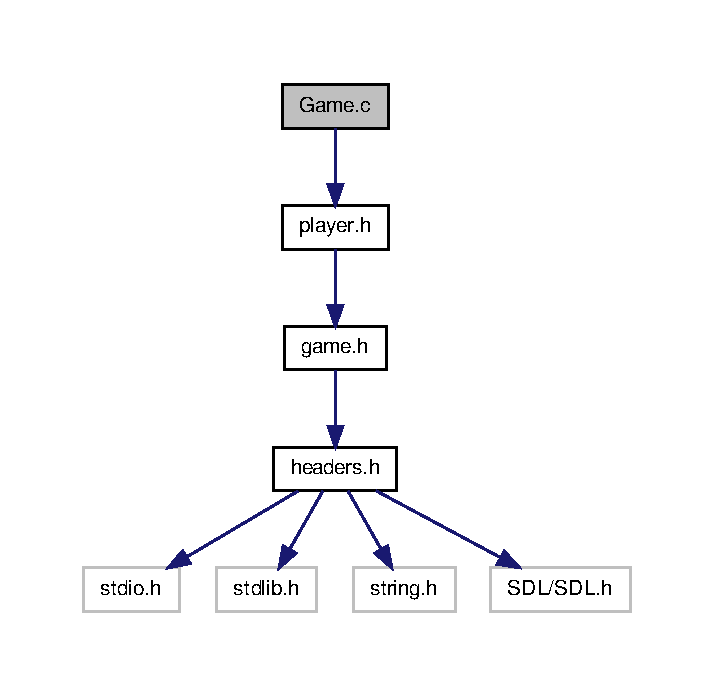
\includegraphics[width=342pt]{_game_8c__incl}
\end{center}
\end{figure}
\subsection*{Definições e Macros}
\begin{DoxyCompactItemize}
\item 
\hypertarget{_game_8c_a864ac6616dfea2db2da5fa7cb56bc814}{
\#define {\bfseries FLECHA}~0}
\label{_game_8c_a864ac6616dfea2db2da5fa7cb56bc814}

\item 
\hypertarget{_game_8c_abe0ec1d45aab5f79cf2ea355a5869890}{
\#define {\bfseries BOMBA}~1}
\label{_game_8c_abe0ec1d45aab5f79cf2ea355a5869890}

\end{DoxyCompactItemize}
\subsection*{Funções}
\begin{DoxyCompactItemize}
\item 
\hypertarget{_game_8c_a1680bc19ec18d037f04ebaa8d7dbed89}{
int {\bfseries Game} (SDL\_\-Surface $\ast$screen)}
\label{_game_8c_a1680bc19ec18d037f04ebaa8d7dbed89}

\item 
\hypertarget{_game_8c_a4f17058b32ebcc5c2195d9a98ae46ad0}{
int {\bfseries newgame} (SDL\_\-Surface $\ast$screen)}
\label{_game_8c_a4f17058b32ebcc5c2195d9a98ae46ad0}

\item 
\hypertarget{_game_8c_a9b2b03b22322472c34ec8868873ca5ae}{
int {\bfseries loadgame} (SDL\_\-Surface $\ast$screen)}
\label{_game_8c_a9b2b03b22322472c34ec8868873ca5ae}

\end{DoxyCompactItemize}


\subsection{Descrição Detalhada}
Função principal do jogo. \begin{DoxyAuthor}{Autor}
João da Silva, Marina Salles, Ricardo Macedo 
\end{DoxyAuthor}

\hypertarget{game_8h}{
\section{Referência do Arquivo game.h}
\label{game_8h}\index{game.h@{game.h}}
}


Headers para unidades e mapa: ataques, movimentos, etc.  


{\ttfamily \#include \char`\"{}headers.h\char`\"{}}\par
Gráfico de dependência de inclusões para game.h:\nopagebreak
\begin{figure}[H]
\begin{center}
\leavevmode
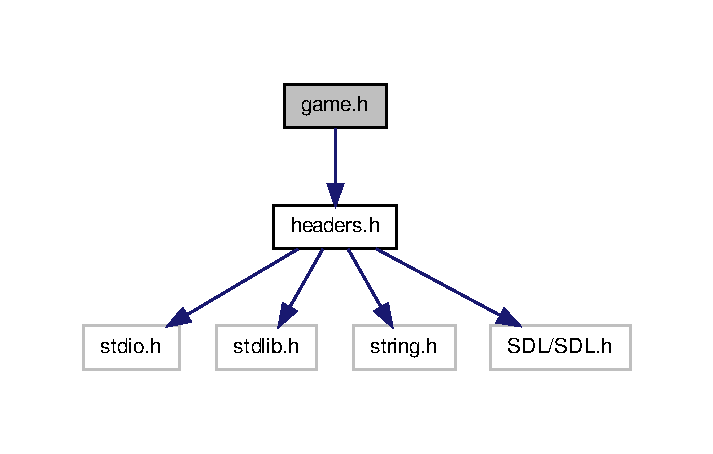
\includegraphics[width=342pt]{game_8h__incl}
\end{center}
\end{figure}
Este grafo mostra quais arquivos estão direta ou indiretamente relacionados com este arquivo:\nopagebreak
\begin{figure}[H]
\begin{center}
\leavevmode
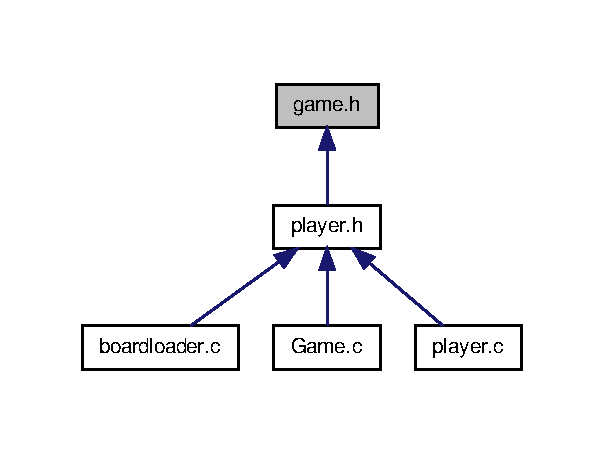
\includegraphics[width=290pt]{game_8h__dep__incl}
\end{center}
\end{figure}
\subsection*{Estruturas de Dados}
\begin{DoxyCompactItemize}
\item 
struct \hyperlink{structvector}{vector}
\item 
struct \hyperlink{structterreno}{terreno}
\item 
struct \hyperlink{structatt}{att}
\item 
struct \hyperlink{structmov}{mov}
\item 
struct \hyperlink{structobj}{obj}
\item 
struct \hyperlink{structgmboard}{gmboard}
\end{DoxyCompactItemize}
\subsection*{Definições e Macros}
\begin{DoxyCompactItemize}
\item 
\hypertarget{game_8h_ae5fc570cf88422a1c5233f5e87ea4cc4}{
\#define {\bfseries MAXATTACKS}~3}
\label{game_8h_ae5fc570cf88422a1c5233f5e87ea4cc4}

\item 
\hypertarget{game_8h_a2e3fa703b74a79159357a228d111c98f}{
\#define {\bfseries MAXIMMUNITIES}~10}
\label{game_8h_a2e3fa703b74a79159357a228d111c98f}

\item 
\hypertarget{game_8h_a21be893fd9b7a79cfe2ab37f064c9403}{
\#define {\bfseries attackType}~int}
\label{game_8h_a21be893fd9b7a79cfe2ab37f064c9403}

\item 
\hypertarget{game_8h_a6db849583506ed57837f9457d40c1cf8}{
\#define {\bfseries ATT\_\-ARROW}~10}
\label{game_8h_a6db849583506ed57837f9457d40c1cf8}

\item 
\hypertarget{game_8h_acbd969a6516e84e3112da752cd0dc274}{
\#define {\bfseries ATT\_\-CANNON}~11}
\label{game_8h_acbd969a6516e84e3112da752cd0dc274}

\item 
\hypertarget{game_8h_acf65ed90a2656632ce60be75a65d861f}{
\#define {\bfseries ATT\_\-TOUCH}~12}
\label{game_8h_acf65ed90a2656632ce60be75a65d861f}

\item 
\hypertarget{game_8h_a701a122c008d563884e4d7ee21d17438}{
\#define {\bfseries ATT\_\-TACKLE}~13}
\label{game_8h_a701a122c008d563884e4d7ee21d17438}

\item 
\hypertarget{game_8h_a51b48ce80e8e6b9d3df0008c38a9bea8}{
\#define {\bfseries ATT\_\-MAGIC}~14}
\label{game_8h_a51b48ce80e8e6b9d3df0008c38a9bea8}

\item 
\hypertarget{game_8h_ad75544f6c49de952a2ab1963368e20c0}{
\#define {\bfseries ATT\_\-SHIP}~16}
\label{game_8h_ad75544f6c49de952a2ab1963368e20c0}

\item 
\hypertarget{game_8h_af5ccccc9e8fe176c3657121389226494}{
\#define {\bfseries ATT\_\-BOMB}~15}
\label{game_8h_af5ccccc9e8fe176c3657121389226494}

\item 
\hypertarget{game_8h_ae32536b7c391d34a9fbce30b1fbc4fb8}{
\#define {\bfseries movementPattern}~int}
\label{game_8h_ae32536b7c391d34a9fbce30b1fbc4fb8}

\item 
\hypertarget{game_8h_abf6fd74fac96e247e3f52f97e9067f79}{
\#define {\bfseries MOV\_\-LINE}~20}
\label{game_8h_abf6fd74fac96e247e3f52f97e9067f79}

\item 
\hypertarget{game_8h_a87891e2ea498a4baa8285795082aad5f}{
\#define {\bfseries MOV\_\-RANDOM}~21}
\label{game_8h_a87891e2ea498a4baa8285795082aad5f}

\item 
\hypertarget{game_8h_ae04a6814bcf4e2a4c61a338260ed9adc}{
\#define {\bfseries MOV\_\-RANDLINES}~22}
\label{game_8h_ae04a6814bcf4e2a4c61a338260ed9adc}

\item 
\hypertarget{game_8h_a6ef4eaee533cc02dd23fce302620671b}{
\#define {\bfseries MOV\_\-NONE}~-\/20}
\label{game_8h_a6ef4eaee533cc02dd23fce302620671b}

\end{DoxyCompactItemize}
\subsection*{Definições de Tipos}
\begin{DoxyCompactItemize}
\item 
\hypertarget{game_8h_a67df6442cbc09def7e2d82c71522e1ae}{
typedef struct \hyperlink{structvector}{vector} {\bfseries Vector}}
\label{game_8h_a67df6442cbc09def7e2d82c71522e1ae}

\item 
\hypertarget{game_8h_ad9f0bb93009117351dc61c52ce5bc203}{
typedef struct \hyperlink{structterreno}{terreno} {\bfseries Terrain}}
\label{game_8h_ad9f0bb93009117351dc61c52ce5bc203}

\item 
\hypertarget{game_8h_a20b7794669e0be47f6ae27f635e9888a}{
typedef struct \hyperlink{structatt}{att} {\bfseries Attack}}
\label{game_8h_a20b7794669e0be47f6ae27f635e9888a}

\item 
\hypertarget{game_8h_a8b9a1d113b7fefcdc535e352867d62fd}{
typedef struct \hyperlink{structmov}{mov} {\bfseries Movement}}
\label{game_8h_a8b9a1d113b7fefcdc535e352867d62fd}

\item 
\hypertarget{game_8h_a5c7504d186628cda40c61cac845c5e1d}{
typedef struct \hyperlink{structobj}{obj} {\bfseries Object}}
\label{game_8h_a5c7504d186628cda40c61cac845c5e1d}

\item 
\hypertarget{game_8h_a20afb84b0cfb61d1263151eaef97465f}{
typedef struct \hyperlink{structgmboard}{gmboard} {\bfseries GameBoard}}
\label{game_8h_a20afb84b0cfb61d1263151eaef97465f}

\end{DoxyCompactItemize}
\subsection*{Funções}
\begin{DoxyCompactItemize}
\item 
void \hyperlink{game_8h_afc079f6d58f20203e10b4eb0e8ea1874}{loadObjectDefinitions} (\hyperlink{structobj}{Object} definitions\mbox{[}$\,$\mbox{]}, char $\ast$filename)
\item 
void \hyperlink{game_8h_a058375b33f392796aaa9049460639426}{loadTerrainDefinitions} (\hyperlink{structterreno}{Terrain} definitions\mbox{[}$\,$\mbox{]}, char $\ast$filename)
\item 
void \hyperlink{game_8h_a4dbeac8b6caf8362bd70531ac1904cbd}{loadObjectDefinition} (\hyperlink{structobj}{Object} $\ast$definition, FILE $\ast$F)
\item 
SDL\_\-Rect $\ast$ \hyperlink{game_8h_a2a1f0038c2fd0907742662aa17566fad}{loadBoard} (\hyperlink{structgmboard}{GameBoard} $\ast$board, \hyperlink{structobj}{Object} definitions\mbox{[}$\,$\mbox{]}, char $\ast$file)
\item 
\hyperlink{structobj}{Object} $\ast$ \hyperlink{game_8h_a522d39ac8eb7f87b05063d2719489bae}{newObject} (char id, \hyperlink{structobj}{Object} defs\mbox{[}$\,$\mbox{]})
\item 
\hyperlink{structobj}{Object} $\ast$ \hyperlink{game_8h_ab2b45b422b800ecc1ed60652267edbc1}{searchObjectDefinition} (char id, \hyperlink{structobj}{Object} defs\mbox{[}$\,$\mbox{]})
\item 
void \hyperlink{game_8h_a52fbb46e4c838dac553df46caaebbc48}{loadMovementInfo} (\hyperlink{structmov}{Movement} $\ast$\hyperlink{structmov}{mov}, FILE $\ast$F)
\item 
void \hyperlink{game_8h_a916135ea4fd3a8e15fb21860686dbf09}{loadAttackInfo} (\hyperlink{structatt}{Attack} $\ast$\hyperlink{structatt}{att}, FILE $\ast$F)
\item 
void \hyperlink{game_8h_a78ef8a82133b9cdffc71f167ebcd3305}{loadImmunitiesInfo} (attackType $\ast$type, FILE $\ast$F)
\item 
void \hyperlink{game_8h_a8fa0c71f272ab9b4cca146f1fe14ec51}{copyObject} (\hyperlink{structobj}{Object} $\ast$new, \hyperlink{structobj}{Object} $\ast$ref)
\item 
void \hyperlink{game_8h_aa6a6de2f0301d872e313fdf5448a823a}{copyMovement} (\hyperlink{structmov}{Movement} $\ast$new, \hyperlink{structmov}{Movement} $\ast$ref)
\item 
void \hyperlink{game_8h_af2e739e0f57149c0581db35571a23290}{copyAttack} (\hyperlink{structatt}{Attack} $\ast$new, \hyperlink{structatt}{Attack} $\ast$ref)
\item 
void \hyperlink{game_8h_a40dd9223c1b66c364eafe63cb2681957}{copyObjectClip} (SDL\_\-Rect $\ast$new, SDL\_\-Rect $\ast$ref)
\item 
\hypertarget{game_8h_a961d9591c97111f68c89816bf4c7374b}{
void {\bfseries fireAttack} (\hyperlink{structgmboard}{GameBoard} $\ast$gameboard, \hyperlink{structobj}{Object} $\ast$attacker, \hyperlink{structvector}{Vector} direction, attackType type)}
\label{game_8h_a961d9591c97111f68c89816bf4c7374b}

\item 
\hypertarget{game_8h_a8f745a5ca2c5247285b39b4db27a8b9b}{
void {\bfseries moveObject} (\hyperlink{structgmboard}{GameBoard} $\ast$gameboard, \hyperlink{structobj}{Object} $\ast$mover)}
\label{game_8h_a8f745a5ca2c5247285b39b4db27a8b9b}

\item 
\hypertarget{game_8h_a71fe52114b66d7e2788ded2a9dccbdd8}{
void {\bfseries updateGameboard} (\hyperlink{structgmboard}{GameBoard} $\ast$gameboard)}
\label{game_8h_a71fe52114b66d7e2788ded2a9dccbdd8}

\end{DoxyCompactItemize}


\subsection{Descrição Detalhada}
Headers para unidades e mapa: ataques, movimentos, etc. \begin{DoxyAuthor}{Autor}
João da Silva, Marina Salles, Ricardo Macedo 
\end{DoxyAuthor}


\subsection{Funções}
\hypertarget{game_8h_af2e739e0f57149c0581db35571a23290}{
\index{game.h@{game.h}!copyAttack@{copyAttack}}
\index{copyAttack@{copyAttack}!game.h@{game.h}}
\subsubsection[{copyAttack}]{\setlength{\rightskip}{0pt plus 5cm}void copyAttack (
\begin{DoxyParamCaption}
\item[{{\bf Attack} $\ast$}]{new, }
\item[{{\bf Attack} $\ast$}]{ref}
\end{DoxyParamCaption}
)}}
\label{game_8h_af2e739e0f57149c0581db35571a23290}
Copia uma estrutura do tipo ataque (usado para copiar objeto) \hypertarget{game_8h_aa6a6de2f0301d872e313fdf5448a823a}{
\index{game.h@{game.h}!copyMovement@{copyMovement}}
\index{copyMovement@{copyMovement}!game.h@{game.h}}
\subsubsection[{copyMovement}]{\setlength{\rightskip}{0pt plus 5cm}void copyMovement (
\begin{DoxyParamCaption}
\item[{{\bf Movement} $\ast$}]{new, }
\item[{{\bf Movement} $\ast$}]{ref}
\end{DoxyParamCaption}
)}}
\label{game_8h_aa6a6de2f0301d872e313fdf5448a823a}
Copia uma estrutura do tipo movimento (usado para copiar objeto) \hypertarget{game_8h_a8fa0c71f272ab9b4cca146f1fe14ec51}{
\index{game.h@{game.h}!copyObject@{copyObject}}
\index{copyObject@{copyObject}!game.h@{game.h}}
\subsubsection[{copyObject}]{\setlength{\rightskip}{0pt plus 5cm}void copyObject (
\begin{DoxyParamCaption}
\item[{{\bf Object} $\ast$}]{new, }
\item[{{\bf Object} $\ast$}]{ref}
\end{DoxyParamCaption}
)}}
\label{game_8h_a8fa0c71f272ab9b4cca146f1fe14ec51}
Copia um Object (usado para criar um objeto a partir das definições) \hypertarget{game_8h_a40dd9223c1b66c364eafe63cb2681957}{
\index{game.h@{game.h}!copyObjectClip@{copyObjectClip}}
\index{copyObjectClip@{copyObjectClip}!game.h@{game.h}}
\subsubsection[{copyObjectClip}]{\setlength{\rightskip}{0pt plus 5cm}void copyObjectClip (
\begin{DoxyParamCaption}
\item[{SDL\_\-Rect $\ast$}]{new, }
\item[{SDL\_\-Rect $\ast$}]{ref}
\end{DoxyParamCaption}
)}}
\label{game_8h_a40dd9223c1b66c364eafe63cb2681957}
Copia um retângulo \hypertarget{game_8h_a916135ea4fd3a8e15fb21860686dbf09}{
\index{game.h@{game.h}!loadAttackInfo@{loadAttackInfo}}
\index{loadAttackInfo@{loadAttackInfo}!game.h@{game.h}}
\subsubsection[{loadAttackInfo}]{\setlength{\rightskip}{0pt plus 5cm}void loadAttackInfo (
\begin{DoxyParamCaption}
\item[{{\bf Attack} $\ast$}]{att, }
\item[{FILE $\ast$}]{F}
\end{DoxyParamCaption}
)}}
\label{game_8h_a916135ea4fd3a8e15fb21860686dbf09}
Carrega informação de ataque do arquivo de dados de objeto \hypertarget{game_8h_a2a1f0038c2fd0907742662aa17566fad}{
\index{game.h@{game.h}!loadBoard@{loadBoard}}
\index{loadBoard@{loadBoard}!game.h@{game.h}}
\subsubsection[{loadBoard}]{\setlength{\rightskip}{0pt plus 5cm}SDL\_\-Rect$\ast$ loadBoard (
\begin{DoxyParamCaption}
\item[{{\bf GameBoard} $\ast$}]{board, }
\item[{{\bf Object}}]{definitions\mbox{[}$\,$\mbox{]}, }
\item[{char $\ast$}]{file}
\end{DoxyParamCaption}
)}}
\label{game_8h_a2a1f0038c2fd0907742662aa17566fad}
Carrega uma fase a partir de um arquivo de fase 
\begin{DoxyParams}{Parâmetros}
{\em board} & Estrutura de dados que guarda as informações do tabuleiro/mapa \\
\hline
{\em definitions} & Estrutura de dados que guarda as definições de objetos \\
\hline
{\em file} & Arquivo de fase \\
\hline
\end{DoxyParams}
\hypertarget{game_8h_a78ef8a82133b9cdffc71f167ebcd3305}{
\index{game.h@{game.h}!loadImmunitiesInfo@{loadImmunitiesInfo}}
\index{loadImmunitiesInfo@{loadImmunitiesInfo}!game.h@{game.h}}
\subsubsection[{loadImmunitiesInfo}]{\setlength{\rightskip}{0pt plus 5cm}void loadImmunitiesInfo (
\begin{DoxyParamCaption}
\item[{attackType $\ast$}]{type, }
\item[{FILE $\ast$}]{F}
\end{DoxyParamCaption}
)}}
\label{game_8h_a78ef8a82133b9cdffc71f167ebcd3305}
Carrega informação de imunidade do arquivo de dados de objeto \hypertarget{game_8h_a52fbb46e4c838dac553df46caaebbc48}{
\index{game.h@{game.h}!loadMovementInfo@{loadMovementInfo}}
\index{loadMovementInfo@{loadMovementInfo}!game.h@{game.h}}
\subsubsection[{loadMovementInfo}]{\setlength{\rightskip}{0pt plus 5cm}void loadMovementInfo (
\begin{DoxyParamCaption}
\item[{{\bf Movement} $\ast$}]{mov, }
\item[{FILE $\ast$}]{F}
\end{DoxyParamCaption}
)}}
\label{game_8h_a52fbb46e4c838dac553df46caaebbc48}
Carrega informação de movimento do arquito de dados de objeto \hypertarget{game_8h_a4dbeac8b6caf8362bd70531ac1904cbd}{
\index{game.h@{game.h}!loadObjectDefinition@{loadObjectDefinition}}
\index{loadObjectDefinition@{loadObjectDefinition}!game.h@{game.h}}
\subsubsection[{loadObjectDefinition}]{\setlength{\rightskip}{0pt plus 5cm}void loadObjectDefinition (
\begin{DoxyParamCaption}
\item[{{\bf Object} $\ast$}]{def, }
\item[{FILE $\ast$}]{F}
\end{DoxyParamCaption}
)}}
\label{game_8h_a4dbeac8b6caf8362bd70531ac1904cbd}
Lê uma linha do arquivo de definições de objetos e carrega um objeto-\/definição para futura referência 
\begin{DoxyParams}{Parâmetros}
{\em def} & Object a ser carregado com a definição \\
\hline
{\em F} & leitor do arquivo de objeto \\
\hline
\end{DoxyParams}
\hypertarget{game_8h_afc079f6d58f20203e10b4eb0e8ea1874}{
\index{game.h@{game.h}!loadObjectDefinitions@{loadObjectDefinitions}}
\index{loadObjectDefinitions@{loadObjectDefinitions}!game.h@{game.h}}
\subsubsection[{loadObjectDefinitions}]{\setlength{\rightskip}{0pt plus 5cm}void loadObjectDefinitions (
\begin{DoxyParamCaption}
\item[{{\bf Object}}]{definitions\mbox{[}$\,$\mbox{]}, }
\item[{char $\ast$}]{filename}
\end{DoxyParamCaption}
)}}
\label{game_8h_afc079f6d58f20203e10b4eb0e8ea1874}
Carrega as definições de objetos de um arquivo de dados 
\begin{DoxyParams}{Parâmetros}
{\em definitions} & Estrutura de dados que armazena as definições \\
\hline
{\em filename} & Nome do arquivo de dados (default: object.dat) \\
\hline
\end{DoxyParams}
\hypertarget{game_8h_a058375b33f392796aaa9049460639426}{
\index{game.h@{game.h}!loadTerrainDefinitions@{loadTerrainDefinitions}}
\index{loadTerrainDefinitions@{loadTerrainDefinitions}!game.h@{game.h}}
\subsubsection[{loadTerrainDefinitions}]{\setlength{\rightskip}{0pt plus 5cm}void loadTerrainDefinitions (
\begin{DoxyParamCaption}
\item[{{\bf Terrain}}]{terrenos\mbox{[}$\,$\mbox{]}, }
\item[{char $\ast$}]{file}
\end{DoxyParamCaption}
)}}
\label{game_8h_a058375b33f392796aaa9049460639426}
Carrega as informações dos elementos de terreno de um arquivo 
\begin{DoxyParams}{Parâmetros}
{\em file} & O arquivo com as informações \\
\hline
{\em terrenos} & O lugar para armazenar as informações \\
\hline
\end{DoxyParams}
\hypertarget{game_8h_a522d39ac8eb7f87b05063d2719489bae}{
\index{game.h@{game.h}!newObject@{newObject}}
\index{newObject@{newObject}!game.h@{game.h}}
\subsubsection[{newObject}]{\setlength{\rightskip}{0pt plus 5cm}{\bf Object}$\ast$ newObject (
\begin{DoxyParamCaption}
\item[{char}]{id, }
\item[{{\bf Object}}]{defs\mbox{[}$\,$\mbox{]}}
\end{DoxyParamCaption}
)}}
\label{game_8h_a522d39ac8eb7f87b05063d2719489bae}
Cria novo objeto, cópia de uma definição 
\begin{DoxyParams}{Parâmetros}
{\em id} & Identificador do tipo de objeto \\
\hline
{\em defs} & Lista de definições \\
\hline
\end{DoxyParams}
\hypertarget{game_8h_ab2b45b422b800ecc1ed60652267edbc1}{
\index{game.h@{game.h}!searchObjectDefinition@{searchObjectDefinition}}
\index{searchObjectDefinition@{searchObjectDefinition}!game.h@{game.h}}
\subsubsection[{searchObjectDefinition}]{\setlength{\rightskip}{0pt plus 5cm}{\bf Object}$\ast$ searchObjectDefinition (
\begin{DoxyParamCaption}
\item[{char}]{id, }
\item[{{\bf Object}}]{defs\mbox{[}$\,$\mbox{]}}
\end{DoxyParamCaption}
)}}
\label{game_8h_ab2b45b422b800ecc1ed60652267edbc1}
Devolve endereço de uma definição 
\begin{DoxyParams}{Parâmetros}
{\em id} & Identificador do tipo de objeto \\
\hline
{\em defs} & Lista de definições \\
\hline
\end{DoxyParams}

\hypertarget{headers_8h}{
\section{Referência do Arquivo headers.h}
\label{headers_8h}\index{headers.h@{headers.h}}
}


Arquivo header geral do jogo, incluindo menu e gráficos.  


{\ttfamily \#include $<$stdio.h$>$}\par
{\ttfamily \#include $<$stdlib.h$>$}\par
{\ttfamily \#include $<$string.h$>$}\par
{\ttfamily \#include \char`\"{}SDL/SDL.h\char`\"{}}\par
Gráfico de dependência de inclusões para headers.h:\nopagebreak
\begin{figure}[H]
\begin{center}
\leavevmode
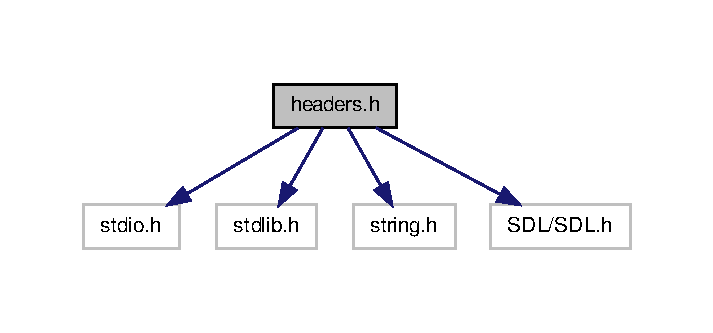
\includegraphics[width=342pt]{headers_8h__incl}
\end{center}
\end{figure}
Este grafo mostra quais arquivos estão direta ou indiretamente relacionados com este arquivo:\nopagebreak
\begin{figure}[H]
\begin{center}
\leavevmode
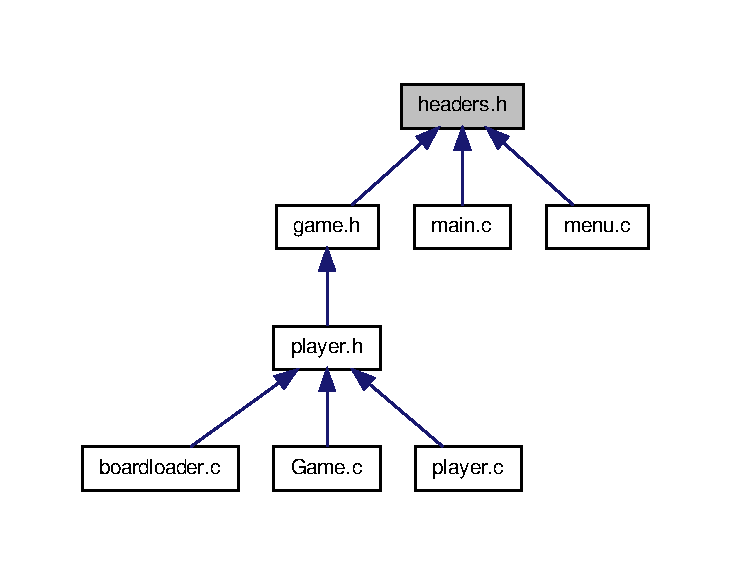
\includegraphics[width=351pt]{headers_8h__dep__incl}
\end{center}
\end{figure}
\subsection*{Definições e Macros}
\begin{DoxyCompactItemize}
\item 
\hypertarget{headers_8h_abb452686968e48b67397da5f97445f5b}{
\#define {\bfseries bool}~int}
\label{headers_8h_abb452686968e48b67397da5f97445f5b}

\item 
\hypertarget{headers_8h_a41f9c5fb8b08eb5dc3edce4dcb37fee7}{
\#define {\bfseries true}~1}
\label{headers_8h_a41f9c5fb8b08eb5dc3edce4dcb37fee7}

\item 
\hypertarget{headers_8h_a65e9886d74aaee76545e83dd09011727}{
\#define {\bfseries false}~0}
\label{headers_8h_a65e9886d74aaee76545e83dd09011727}

\item 
\hypertarget{headers_8h_ae6648cd71a8bd49d58ae8ed33ba910d1}{
\#define {\bfseries MAXLEN}~100}
\label{headers_8h_ae6648cd71a8bd49d58ae8ed33ba910d1}

\item 
\hypertarget{headers_8h_ad24e2b54375e12474e65ebf7175988fb}{
\#define {\bfseries QUIT}~-\/1}
\label{headers_8h_ad24e2b54375e12474e65ebf7175988fb}

\item 
\hypertarget{headers_8h_a0cfd5d3f47cf0b1f532c667efa58ec77}{
\#define {\bfseries IMAGEDIR}~\char`\"{}data/imagens/\char`\"{}}
\label{headers_8h_a0cfd5d3f47cf0b1f532c667efa58ec77}

\item 
\hypertarget{headers_8h_a2cd109632a6dcccaa80b43561b1ab700}{
\#define {\bfseries SCREEN\_\-WIDTH}~(48$\ast$15)}
\label{headers_8h_a2cd109632a6dcccaa80b43561b1ab700}

\item 
\hypertarget{headers_8h_a6974d08a74da681b3957b2fead2608b8}{
\#define {\bfseries SCREEN\_\-HEIGHT}~480}
\label{headers_8h_a6974d08a74da681b3957b2fead2608b8}

\item 
\hypertarget{headers_8h_a95d55ebfa2f2f1bd14867ad6a6cc9bfb}{
\#define {\bfseries RESOLUTION}~24}
\label{headers_8h_a95d55ebfa2f2f1bd14867ad6a6cc9bfb}

\item 
\hypertarget{headers_8h_afa556a68b7c0fcc58cd87c5f36859f30}{
\#define {\bfseries BR}~0}
\label{headers_8h_afa556a68b7c0fcc58cd87c5f36859f30}

\item 
\hypertarget{headers_8h_ab05cfd0a3a5e9ed76d38482e2cd26f9f}{
\#define {\bfseries BG}~0xFF}
\label{headers_8h_ab05cfd0a3a5e9ed76d38482e2cd26f9f}

\item 
\hypertarget{headers_8h_ad91fa5bb7926a489c6e63eb6f6ca4a19}{
\#define {\bfseries BB}~0xFF}
\label{headers_8h_ad91fa5bb7926a489c6e63eb6f6ca4a19}

\item 
\hypertarget{headers_8h_a76108891dc4352082a676f2978ee446d}{
\#define {\bfseries TILE\_\-WIDTH}~48}
\label{headers_8h_a76108891dc4352082a676f2978ee446d}

\item 
\hypertarget{headers_8h_a74b119c5bb38a697fc531b7b86fb0a54}{
\#define {\bfseries TILE\_\-HEIGHT}~48}
\label{headers_8h_a74b119c5bb38a697fc531b7b86fb0a54}

\item 
\hypertarget{headers_8h_a1cd139e8d1f7ae83f54c8d477313d8ea}{
\#define {\bfseries BOARD\_\-WIDTH}~15}
\label{headers_8h_a1cd139e8d1f7ae83f54c8d477313d8ea}

\item 
\hypertarget{headers_8h_a94ed08e31d2f3a38d35f0cb89c762f04}{
\#define {\bfseries BOARD\_\-HEIGHT}~10}
\label{headers_8h_a94ed08e31d2f3a38d35f0cb89c762f04}

\item 
\hypertarget{headers_8h_a17897dbbc6ff46c90212d087f60f38c4}{
\#define {\bfseries DATADIR}~\char`\"{}data/\char`\"{}}
\label{headers_8h_a17897dbbc6ff46c90212d087f60f38c4}

\item 
\hypertarget{headers_8h_ac7d60a97ab67b251d5ddfed2cc51ee8d}{
\#define {\bfseries NEWGAME}~0}
\label{headers_8h_ac7d60a97ab67b251d5ddfed2cc51ee8d}

\item 
\hypertarget{headers_8h_af727c65f29aaa8a4115479768590819e}{
\#define {\bfseries LOADGAME}~1}
\label{headers_8h_af727c65f29aaa8a4115479768590819e}

\item 
\hypertarget{headers_8h_aec95ee3aec6673f51ed3c6a833a2dc71}{
\#define {\bfseries OPTIONS}~2}
\label{headers_8h_aec95ee3aec6673f51ed3c6a833a2dc71}

\item 
\hypertarget{headers_8h_a8187a9af791c0a44ba67edd9cf266961}{
\#define {\bfseries MANUAL}~3}
\label{headers_8h_a8187a9af791c0a44ba67edd9cf266961}

\item 
\hypertarget{headers_8h_a28017dea6f5becdb38eba6eac6f51bbc}{
\#define {\bfseries CREDITS}~4}
\label{headers_8h_a28017dea6f5becdb38eba6eac6f51bbc}

\item 
\hypertarget{headers_8h_a60a56c499875b57369f7ef3a5a227cb9}{
\#define {\bfseries TITLE}~5}
\label{headers_8h_a60a56c499875b57369f7ef3a5a227cb9}

\item 
\hypertarget{headers_8h_ac90300e1e2bc5e5b092407b9c5267c9a}{
\#define {\bfseries COMMANDS}~6}
\label{headers_8h_ac90300e1e2bc5e5b092407b9c5267c9a}

\end{DoxyCompactItemize}
\subsection*{Funções}
\begin{DoxyCompactItemize}
\item 
SDL\_\-Surface $\ast$ \hyperlink{headers_8h_a69fd26d27992269d2bf768c2d6d885cc}{initScreen} (int largura, int altura)
\item 
SDL\_\-Surface $\ast$ \hyperlink{headers_8h_a263da16929f6ea3d596249c06da671ad}{loadBMP} (char $\ast$file)
\item 
void \hyperlink{headers_8h_af439732bba4b3a81495c9460ae57b734}{applySurface} (SDL\_\-Surface $\ast$destination, SDL\_\-Surface $\ast$source)
\item 
void \hyperlink{headers_8h_aec41560888e5d758a2a1d6a08436859d}{applyDoubleInfoClip} (SDL\_\-Surface $\ast$destination, SDL\_\-Surface $\ast$source, SDL\_\-Rect clip\mbox{[}$\,$\mbox{]}\mbox{[}2\mbox{]}, int choice)
\item 
void \hyperlink{headers_8h_a8a7df9bbda68e46b75a2bdf2056c870d}{loadDoubleInfoClip} (char $\ast$file, SDL\_\-Rect clip\mbox{[}$\,$\mbox{]}\mbox{[}2\mbox{]})
\item 
\hypertarget{headers_8h_a0ac6a35818a1ebdb166959fad63d4d32}{
void {\bfseries applyClip} (SDL\_\-Surface $\ast$destination, SDL\_\-Surface $\ast$source, int x, int y, SDL\_\-Rect clip)}
\label{headers_8h_a0ac6a35818a1ebdb166959fad63d4d32}

\item 
void \hyperlink{headers_8h_ad2fc94e1c6dbf5ef17a9ac286c8cceaf}{applyClipToBoard} (SDL\_\-Surface $\ast$destination, SDL\_\-Surface $\ast$source, int board\_\-x, int board\_\-y, SDL\_\-Rect clip)
\item 
void \hyperlink{headers_8h_ac1069ac1fdef17f65759ecd6819a0f11}{safeFreeSurface} (SDL\_\-Surface $\ast$dead)
\item 
void \hyperlink{headers_8h_a54ce253826e283991f35d6a97d346a46}{gunther\_\-menu} (SDL\_\-Surface $\ast$screen)
\item 
\hypertarget{headers_8h_af26f6b5c02e28bd5037ef7ee6dc2e2cf}{
int {\bfseries intro} (SDL\_\-Surface $\ast$screen)}
\label{headers_8h_af26f6b5c02e28bd5037ef7ee6dc2e2cf}

\item 
int \hyperlink{headers_8h_a79fb862d32102adb3afd6c4850efa80f}{title} (SDL\_\-Surface $\ast$screen)
\item 
\hypertarget{headers_8h_a7d1a4254bb9ad756b0528b4c95be9443}{
int {\bfseries options} (SDL\_\-Surface $\ast$screen)}
\label{headers_8h_a7d1a4254bb9ad756b0528b4c95be9443}

\item 
int \hyperlink{headers_8h_af3231d0d69b075fdf6a3fffc4e05f50b}{manual} (SDL\_\-Surface $\ast$screen, int section)
\item 
\hypertarget{headers_8h_a10e82c49851064a9aae3397425f5b936}{
int {\bfseries credits} (SDL\_\-Surface $\ast$screen)}
\label{headers_8h_a10e82c49851064a9aae3397425f5b936}

\item 
\hypertarget{headers_8h_a9b2b03b22322472c34ec8868873ca5ae}{
int {\bfseries loadgame} (SDL\_\-Surface $\ast$screen)}
\label{headers_8h_a9b2b03b22322472c34ec8868873ca5ae}

\item 
\hypertarget{headers_8h_a4f17058b32ebcc5c2195d9a98ae46ad0}{
int {\bfseries newgame} (SDL\_\-Surface $\ast$screen)}
\label{headers_8h_a4f17058b32ebcc5c2195d9a98ae46ad0}

\end{DoxyCompactItemize}


\subsection{Descrição Detalhada}
Arquivo header geral do jogo, incluindo menu e gráficos. \begin{DoxyAuthor}{Autor}
João da Silva, Marina Salles, Ricardo Macedo 
\end{DoxyAuthor}


\subsection{Funções}
\hypertarget{headers_8h_ad2fc94e1c6dbf5ef17a9ac286c8cceaf}{
\index{headers.h@{headers.h}!applyClipToBoard@{applyClipToBoard}}
\index{applyClipToBoard@{applyClipToBoard}!headers.h@{headers.h}}
\subsubsection[{applyClipToBoard}]{\setlength{\rightskip}{0pt plus 5cm}void applyClipToBoard (
\begin{DoxyParamCaption}
\item[{SDL\_\-Surface $\ast$}]{destination, }
\item[{SDL\_\-Surface $\ast$}]{source, }
\item[{int}]{board\_\-x, }
\item[{int}]{board\_\-y, }
\item[{SDL\_\-Rect}]{clip}
\end{DoxyParamCaption}
)}}
\label{headers_8h_ad2fc94e1c6dbf5ef17a9ac286c8cceaf}
Aplica um retângulo a uma tela 
\begin{DoxyParams}{Parâmetros}
{\em destino} & A tela que receberá a imagem \\
\hline
{\em origem} & A tela de origem \\
\hline
{\em mapa\_\-x} & A posição X (em ladrilhos) no destino \\
\hline
{\em mapa\_\-y} & A posição Y (em ladrilhos) no destino \\
\hline
{\em clip} & O retângulo a ser aplicado \\
\hline
\end{DoxyParams}
\hypertarget{headers_8h_aec41560888e5d758a2a1d6a08436859d}{
\index{headers.h@{headers.h}!applyDoubleInfoClip@{applyDoubleInfoClip}}
\index{applyDoubleInfoClip@{applyDoubleInfoClip}!headers.h@{headers.h}}
\subsubsection[{applyDoubleInfoClip}]{\setlength{\rightskip}{0pt plus 5cm}void applyDoubleInfoClip (
\begin{DoxyParamCaption}
\item[{SDL\_\-Surface $\ast$}]{destination, }
\item[{SDL\_\-Surface $\ast$}]{source, }
\item[{SDL\_\-Rect}]{clip\mbox{[}$\,$\mbox{]}\mbox{[}2\mbox{]}, }
\item[{int}]{choice}
\end{DoxyParamCaption}
)}}
\label{headers_8h_aec41560888e5d758a2a1d6a08436859d}
Copia um retângulo em uma tela para um outro retângulo em outra tela 
\begin{DoxyParams}{Parâmetros}
{\em destino} & Tela de destino \\
\hline
{\em origem} & Tela de origem \\
\hline
{\em clip} & Vetor com os retângulos \\
\hline
{\em selecao} & Opção selecionada no menu \\
\hline
\end{DoxyParams}
\hypertarget{headers_8h_af439732bba4b3a81495c9460ae57b734}{
\index{headers.h@{headers.h}!applySurface@{applySurface}}
\index{applySurface@{applySurface}!headers.h@{headers.h}}
\subsubsection[{applySurface}]{\setlength{\rightskip}{0pt plus 5cm}void applySurface (
\begin{DoxyParamCaption}
\item[{SDL\_\-Surface $\ast$}]{destination, }
\item[{SDL\_\-Surface $\ast$}]{source}
\end{DoxyParamCaption}
)}}
\label{headers_8h_af439732bba4b3a81495c9460ae57b734}
Aplica uma tela guardada em memória em outra 
\begin{DoxyParams}{Parâmetros}
{\em destino} & Tela de destino \\
\hline
{\em origem} & Tela de origem \\
\hline
\end{DoxyParams}
\hypertarget{headers_8h_a54ce253826e283991f35d6a97d346a46}{
\index{headers.h@{headers.h}!gunther\_\-menu@{gunther\_\-menu}}
\index{gunther\_\-menu@{gunther\_\-menu}!headers.h@{headers.h}}
\subsubsection[{gunther\_\-menu}]{\setlength{\rightskip}{0pt plus 5cm}void gunther\_\-menu (
\begin{DoxyParamCaption}
\item[{SDL\_\-Surface $\ast$}]{screen}
\end{DoxyParamCaption}
)}}
\label{headers_8h_a54ce253826e283991f35d6a97d346a46}
Renderiza o menu baseado na seleção 
\begin{DoxyParams}{Parâmetros}
{\em tela} & Tela onde o menu será renderizado \\
\hline
\end{DoxyParams}
\hypertarget{headers_8h_a69fd26d27992269d2bf768c2d6d885cc}{
\index{headers.h@{headers.h}!initScreen@{initScreen}}
\index{initScreen@{initScreen}!headers.h@{headers.h}}
\subsubsection[{initScreen}]{\setlength{\rightskip}{0pt plus 5cm}SDL\_\-Surface$\ast$ initScreen (
\begin{DoxyParamCaption}
\item[{int}]{largura, }
\item[{int}]{altura}
\end{DoxyParamCaption}
)}}
\label{headers_8h_a69fd26d27992269d2bf768c2d6d885cc}
Abre uma nova janela 
\begin{DoxyParams}{Parâmetros}
{\em largura} & Largura em pixels \\
\hline
{\em altura} & Altura em pixels \\
\hline
\end{DoxyParams}
\hypertarget{headers_8h_a263da16929f6ea3d596249c06da671ad}{
\index{headers.h@{headers.h}!loadBMP@{loadBMP}}
\index{loadBMP@{loadBMP}!headers.h@{headers.h}}
\subsubsection[{loadBMP}]{\setlength{\rightskip}{0pt plus 5cm}SDL\_\-Surface$\ast$ loadBMP (
\begin{DoxyParamCaption}
\item[{char $\ast$}]{file}
\end{DoxyParamCaption}
)}}
\label{headers_8h_a263da16929f6ea3d596249c06da671ad}
Carrega um arquivo Bitmap em uma tela 
\begin{DoxyParams}{Parâmetros}
{\em arquivo} & O nome do arquivo \\
\hline
\end{DoxyParams}
\hypertarget{headers_8h_a8a7df9bbda68e46b75a2bdf2056c870d}{
\index{headers.h@{headers.h}!loadDoubleInfoClip@{loadDoubleInfoClip}}
\index{loadDoubleInfoClip@{loadDoubleInfoClip}!headers.h@{headers.h}}
\subsubsection[{loadDoubleInfoClip}]{\setlength{\rightskip}{0pt plus 5cm}void loadDoubleInfoClip (
\begin{DoxyParamCaption}
\item[{char $\ast$}]{file, }
\item[{SDL\_\-Rect}]{clip\mbox{[}$\,$\mbox{]}\mbox{[}2\mbox{]}}
\end{DoxyParamCaption}
)}}
\label{headers_8h_a8a7df9bbda68e46b75a2bdf2056c870d}
Carrega retângulos a partir de um arquivo 
\begin{DoxyParams}{Parâmetros}
{\em arquivo} & O arquivo a ser carregado \\
\hline
{\em clip} & O vetor de retângulos que conterá as informações \\
\hline
\end{DoxyParams}
\hypertarget{headers_8h_af3231d0d69b075fdf6a3fffc4e05f50b}{
\index{headers.h@{headers.h}!manual@{manual}}
\index{manual@{manual}!headers.h@{headers.h}}
\subsubsection[{manual}]{\setlength{\rightskip}{0pt plus 5cm}int manual (
\begin{DoxyParamCaption}
\item[{SDL\_\-Surface $\ast$}]{screen, }
\item[{int}]{mode}
\end{DoxyParamCaption}
)}}
\label{headers_8h_af3231d0d69b075fdf6a3fffc4e05f50b}
Seção \char`\"{}Manual\char`\"{} do menu 
\begin{DoxyParams}{Parâmetros}
{\em tela} & Tela onde a seção será renderizada \\
\hline
\end{DoxyParams}
\hypertarget{headers_8h_ac1069ac1fdef17f65759ecd6819a0f11}{
\index{headers.h@{headers.h}!safeFreeSurface@{safeFreeSurface}}
\index{safeFreeSurface@{safeFreeSurface}!headers.h@{headers.h}}
\subsubsection[{safeFreeSurface}]{\setlength{\rightskip}{0pt plus 5cm}void safeFreeSurface (
\begin{DoxyParamCaption}
\item[{SDL\_\-Surface $\ast$}]{dead}
\end{DoxyParamCaption}
)}}
\label{headers_8h_ac1069ac1fdef17f65759ecd6819a0f11}
Libera a memória de uma tela 
\begin{DoxyParams}{Parâmetros}
{\em tela} & A tela em questão \\
\hline
\end{DoxyParams}
\hypertarget{headers_8h_a79fb862d32102adb3afd6c4850efa80f}{
\index{headers.h@{headers.h}!title@{title}}
\index{title@{title}!headers.h@{headers.h}}
\subsubsection[{title}]{\setlength{\rightskip}{0pt plus 5cm}int title (
\begin{DoxyParamCaption}
\item[{SDL\_\-Surface $\ast$}]{screen}
\end{DoxyParamCaption}
)}}
\label{headers_8h_a79fb862d32102adb3afd6c4850efa80f}
Menu principal 
\begin{DoxyParams}{Parâmetros}
{\em tela} & Tela onde o menu será renderizado \\
\hline
\end{DoxyParams}

\hypertarget{main_8c}{\section{src/main.c File Reference}
\label{main_8c}\index{src/main.\-c@{src/main.\-c}}
}


Este é o arquivo que implementa as funções descritas na \hyperlink{fisica_8c}{fisica.\-c}. Aqui, carrega-\/se um arquivo texto com as condições iniciais e escreve um arquivo \char`\"{}saida.\-out\char`\"{} com as informações após as iterações.  


{\ttfamily \#include $<$stdio.\-h$>$}\\*
{\ttfamily \#include $<$stdlib.\-h$>$}\\*
{\ttfamily \#include $<$string.\-h$>$}\\*
{\ttfamily \#include \char`\"{}../include/rketypes.\-h\char`\"{}}\\*
{\ttfamily \#include \char`\"{}../include/rkefisica.\-h\char`\"{}}\\*
Include dependency graph for main.\-c\-:
\subsection*{Functions}
\begin{DoxyCompactItemize}
\item 
\hypertarget{main_8c_a0ddf1224851353fc92bfbff6f499fa97}{int {\bfseries main} (int argc, char $\ast$argv\mbox{[}$\,$\mbox{]})}\label{main_8c_a0ddf1224851353fc92bfbff6f499fa97}

\end{DoxyCompactItemize}


\subsection{Detailed Description}
Este é o arquivo que implementa as funções descritas na \hyperlink{fisica_8c}{fisica.\-c}. Aqui, carrega-\/se um arquivo texto com as condições iniciais e escreve um arquivo \char`\"{}saida.\-out\char`\"{} com as informações após as iterações. \begin{DoxyAuthor}{Author}
João da Silva, Marina Salles, Ricardo Macedo 
\end{DoxyAuthor}

\hypertarget{menu_8c}{
\section{Referência do Arquivo menu.c}
\label{menu_8c}\index{menu.c@{menu.c}}
}


Implementação do menu principal.  


{\ttfamily \#include \char`\"{}headers.h\char`\"{}}\par
Gráfico de dependência de inclusões para menu.c:\nopagebreak
\begin{figure}[H]
\begin{center}
\leavevmode
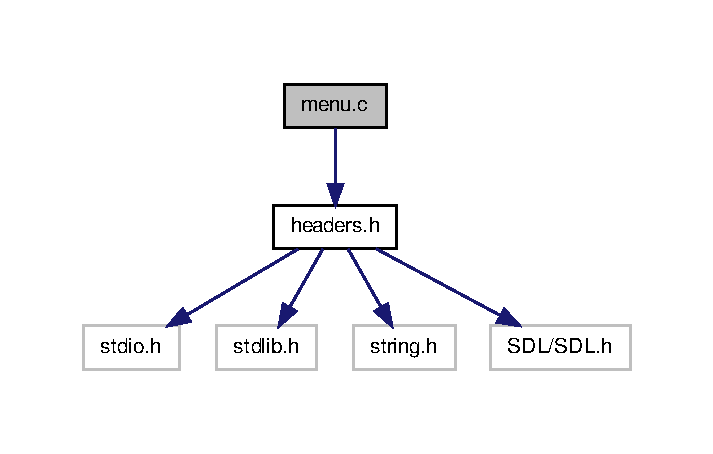
\includegraphics[width=342pt]{menu_8c__incl}
\end{center}
\end{figure}
\subsection*{Funções}
\begin{DoxyCompactItemize}
\item 
void \hyperlink{menu_8c_a54ce253826e283991f35d6a97d346a46}{gunther\_\-menu} (SDL\_\-Surface $\ast$screen)
\item 
int \hyperlink{menu_8c_a79fb862d32102adb3afd6c4850efa80f}{title} (SDL\_\-Surface $\ast$screen)
\item 
int \hyperlink{menu_8c_a4f64a22b2d93a0825625d69dec8b5524}{manual} (SDL\_\-Surface $\ast$screen, int mode)
\item 
\hypertarget{menu_8c_a7d1a4254bb9ad756b0528b4c95be9443}{
int {\bfseries options} (SDL\_\-Surface $\ast$screen)}
\label{menu_8c_a7d1a4254bb9ad756b0528b4c95be9443}

\item 
\hypertarget{menu_8c_af26f6b5c02e28bd5037ef7ee6dc2e2cf}{
int {\bfseries intro} (SDL\_\-Surface $\ast$screen)}
\label{menu_8c_af26f6b5c02e28bd5037ef7ee6dc2e2cf}

\item 
\hypertarget{menu_8c_a10e82c49851064a9aae3397425f5b936}{
int {\bfseries credits} (SDL\_\-Surface $\ast$screen)}
\label{menu_8c_a10e82c49851064a9aae3397425f5b936}

\end{DoxyCompactItemize}


\subsection{Descrição Detalhada}
Implementação do menu principal. \begin{DoxyAuthor}{Autor}
João da Silva, Marina Salles, Ricardo Macedo 
\end{DoxyAuthor}


\subsection{Funções}
\hypertarget{menu_8c_a54ce253826e283991f35d6a97d346a46}{
\index{menu.c@{menu.c}!gunther\_\-menu@{gunther\_\-menu}}
\index{gunther\_\-menu@{gunther\_\-menu}!menu.c@{menu.c}}
\subsubsection[{gunther\_\-menu}]{\setlength{\rightskip}{0pt plus 5cm}void gunther\_\-menu (
\begin{DoxyParamCaption}
\item[{SDL\_\-Surface $\ast$}]{screen}
\end{DoxyParamCaption}
)}}
\label{menu_8c_a54ce253826e283991f35d6a97d346a46}
Renderiza o menu baseado na seleção 
\begin{DoxyParams}{Parâmetros}
{\em tela} & Tela onde o menu será renderizado \\
\hline
\end{DoxyParams}
\hypertarget{menu_8c_a4f64a22b2d93a0825625d69dec8b5524}{
\index{menu.c@{menu.c}!manual@{manual}}
\index{manual@{manual}!menu.c@{menu.c}}
\subsubsection[{manual}]{\setlength{\rightskip}{0pt plus 5cm}int manual (
\begin{DoxyParamCaption}
\item[{SDL\_\-Surface $\ast$}]{screen, }
\item[{int}]{mode}
\end{DoxyParamCaption}
)}}
\label{menu_8c_a4f64a22b2d93a0825625d69dec8b5524}
Seção \char`\"{}Manual\char`\"{} do menu 
\begin{DoxyParams}{Parâmetros}
{\em tela} & Tela onde a seção será renderizada \\
\hline
\end{DoxyParams}
\hypertarget{menu_8c_a79fb862d32102adb3afd6c4850efa80f}{
\index{menu.c@{menu.c}!title@{title}}
\index{title@{title}!menu.c@{menu.c}}
\subsubsection[{title}]{\setlength{\rightskip}{0pt plus 5cm}int title (
\begin{DoxyParamCaption}
\item[{SDL\_\-Surface $\ast$}]{screen}
\end{DoxyParamCaption}
)}}
\label{menu_8c_a79fb862d32102adb3afd6c4850efa80f}
Menu principal 
\begin{DoxyParams}{Parâmetros}
{\em tela} & Tela onde o menu será renderizado \\
\hline
\end{DoxyParams}

\hypertarget{player_8c}{
\section{Referência do Arquivo player.c}
\label{player_8c}\index{player.c@{player.c}}
}


Código para o jogador: imagens, ataques, movimentos, comandos, etc.  


{\ttfamily \#include \char`\"{}player.h\char`\"{}}\par
Gráfico de dependência de inclusões para player.c:\nopagebreak
\begin{figure}[H]
\begin{center}
\leavevmode
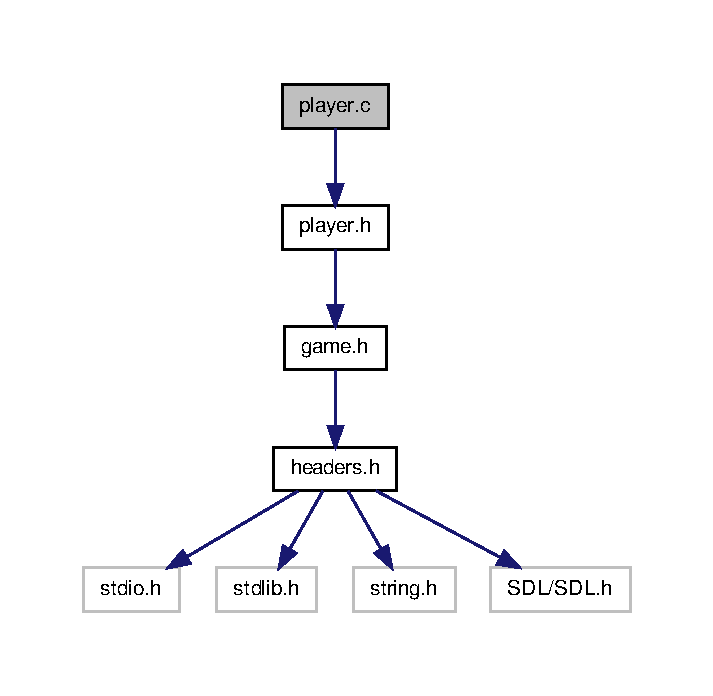
\includegraphics[width=342pt]{player_8c__incl}
\end{center}
\end{figure}
\subsection*{Funções}
\begin{DoxyCompactItemize}
\item 
void \hyperlink{player_8c_a367aed7c3de5f557a25d934be4aee8a4}{rke\_\-carrega\_\-jogador} (\hyperlink{struct__jogador}{Jogador} $\ast$jogador, int larg\_\-ladrilho, int alt\_\-ladrilho)
\item 
void \hyperlink{player_8c_a16dbdc2e1ba993cc3b577143b292252f}{rke\_\-move\_\-jogador} (\hyperlink{struct__jogador}{Jogador} $\ast$jogador, \hyperlink{structgmboard}{GameBoard} tabuleiro, \hyperlink{structterreno}{Terrain} $\ast$terrenos, \hyperlink{structobj}{Object} $\ast$objetos, int delta\_\-x, int delta\_\-y)
\item 
void \hyperlink{player_8c_af58d7aad09f5ab9f3c4ca221436be2cd}{rke\_\-jogador\_\-atira} (\hyperlink{struct__jogador}{Jogador} $\ast$jogador, \hyperlink{structgmboard}{GameBoard} tabuleiro, \hyperlink{structterreno}{Terrain} $\ast$terrenos, \hyperlink{structobj}{Object} $\ast$objetos, int bomba)
\end{DoxyCompactItemize}


\subsection{Descrição Detalhada}
Código para o jogador: imagens, ataques, movimentos, comandos, etc. \begin{DoxyAuthor}{Autor}
João da Silva, Marina Salles, Ricardo Macedo 
\end{DoxyAuthor}


\subsection{Funções}
\hypertarget{player_8c_a367aed7c3de5f557a25d934be4aee8a4}{
\index{player.c@{player.c}!rke\_\-carrega\_\-jogador@{rke\_\-carrega\_\-jogador}}
\index{rke\_\-carrega\_\-jogador@{rke\_\-carrega\_\-jogador}!player.c@{player.c}}
\subsubsection[{rke\_\-carrega\_\-jogador}]{\setlength{\rightskip}{0pt plus 5cm}void rke\_\-carrega\_\-jogador (
\begin{DoxyParamCaption}
\item[{{\bf Jogador} $\ast$}]{jogador, }
\item[{int}]{larg\_\-ladrilho, }
\item[{int}]{alt\_\-ladrilho}
\end{DoxyParamCaption}
)}}
\label{player_8c_a367aed7c3de5f557a25d934be4aee8a4}
Carrega os retângulos da imagem do jogador 
\begin{DoxyParams}{Parâmetros}
{\em O} & lugar para armazenar as informações \\
\hline
{\em Largura} & em pixels do ladrilho \\
\hline
{\em Altura} & em pixels do ladrilho \\
\hline
\end{DoxyParams}
\hypertarget{player_8c_af58d7aad09f5ab9f3c4ca221436be2cd}{
\index{player.c@{player.c}!rke\_\-jogador\_\-atira@{rke\_\-jogador\_\-atira}}
\index{rke\_\-jogador\_\-atira@{rke\_\-jogador\_\-atira}!player.c@{player.c}}
\subsubsection[{rke\_\-jogador\_\-atira}]{\setlength{\rightskip}{0pt plus 5cm}void rke\_\-jogador\_\-atira (
\begin{DoxyParamCaption}
\item[{{\bf Jogador} $\ast$}]{jogador, }
\item[{{\bf GameBoard}}]{tabuleiro, }
\item[{{\bf Terrain} $\ast$}]{terrenos, }
\item[{{\bf Object} $\ast$}]{objetos, }
\item[{int}]{bomba}
\end{DoxyParamCaption}
)}}
\label{player_8c_af58d7aad09f5ab9f3c4ca221436be2cd}
Função de acao de atirar do jogador. 
\begin{DoxyParams}{Parâmetros}
{\em jogador} & Informações do jogador \\
\hline
{\em tabuleiro} & Informações do tabuleiro \\
\hline
{\em terrenos} & Informações dos elementos de terreno \\
\hline
{\em objetos} & Informações dos objetos \\
\hline
\end{DoxyParams}
\hypertarget{player_8c_a16dbdc2e1ba993cc3b577143b292252f}{
\index{player.c@{player.c}!rke\_\-move\_\-jogador@{rke\_\-move\_\-jogador}}
\index{rke\_\-move\_\-jogador@{rke\_\-move\_\-jogador}!player.c@{player.c}}
\subsubsection[{rke\_\-move\_\-jogador}]{\setlength{\rightskip}{0pt plus 5cm}void rke\_\-move\_\-jogador (
\begin{DoxyParamCaption}
\item[{{\bf Jogador} $\ast$}]{jogador, }
\item[{{\bf GameBoard}}]{tabuleiro, }
\item[{{\bf Terrain} $\ast$}]{terrenos, }
\item[{{\bf Object} $\ast$}]{objetos, }
\item[{int}]{delta\_\-x, }
\item[{int}]{delta\_\-y}
\end{DoxyParamCaption}
)}}
\label{player_8c_a16dbdc2e1ba993cc3b577143b292252f}
Função de movimentação do jogador. 
\begin{DoxyParams}{Parâmetros}
{\em jogador} & Informações do jogador \\
\hline
{\em tabuleiro} & Informações do tabuleiro \\
\hline
{\em terrenos} & Informações dos elementos de terreno \\
\hline
{\em objetos} & Informações dos objetos \\
\hline
{\em delta\_\-x} & Movimentação no eixo X \\
\hline
{\em delta\_\-y} & Movimentação no eixo Y \\
\hline
\end{DoxyParams}

\hypertarget{player_8h}{
\section{Referência do Arquivo player.h}
\label{player_8h}\index{player.h@{player.h}}
}


Header para o jogador: imagens, ataques, movimentos, comandos, etc.  


{\ttfamily \#include \char`\"{}game.h\char`\"{}}\par
Gráfico de dependência de inclusões para player.h:\nopagebreak
\begin{figure}[H]
\begin{center}
\leavevmode
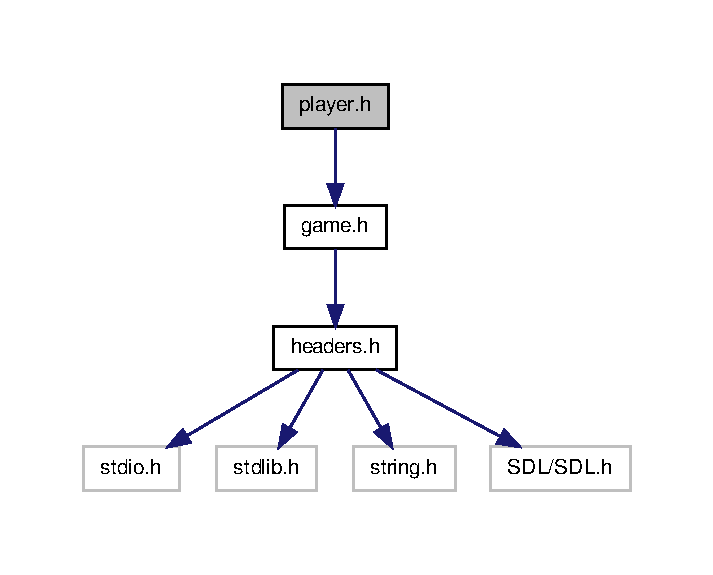
\includegraphics[width=342pt]{player_8h__incl}
\end{center}
\end{figure}
Este grafo mostra quais arquivos estão direta ou indiretamente relacionados com este arquivo:\nopagebreak
\begin{figure}[H]
\begin{center}
\leavevmode
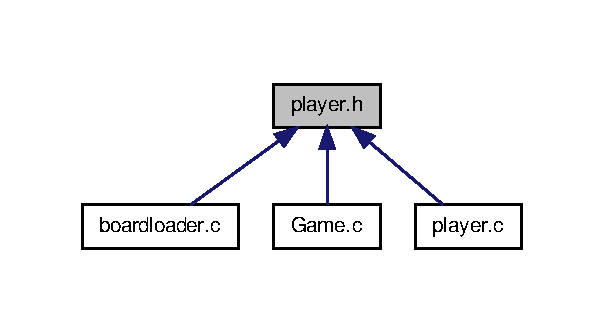
\includegraphics[width=290pt]{player_8h__dep__incl}
\end{center}
\end{figure}
\subsection*{Estruturas de Dados}
\begin{DoxyCompactItemize}
\item 
struct \hyperlink{struct__jogador}{\_\-jogador}
\end{DoxyCompactItemize}
\subsection*{Definições e Macros}
\begin{DoxyCompactItemize}
\item 
\hypertarget{player_8h_a0240ac851181b84ac374872dc5434ee4}{
\#define {\bfseries N}~0}
\label{player_8h_a0240ac851181b84ac374872dc5434ee4}

\item 
\hypertarget{player_8h_a5af9139e882aef6c820ae908589a40d6}{
\#define {\bfseries NE}~1}
\label{player_8h_a5af9139e882aef6c820ae908589a40d6}

\item 
\hypertarget{player_8h_a07484107e6d9fdf38b53edf631d6511d}{
\#define {\bfseries E}~2}
\label{player_8h_a07484107e6d9fdf38b53edf631d6511d}

\item 
\hypertarget{player_8h_a18bbe716f5be6adbd2150139244c0262}{
\#define {\bfseries SE}~3}
\label{player_8h_a18bbe716f5be6adbd2150139244c0262}

\item 
\hypertarget{player_8h_af933676109efed7ab34cea71d748a517}{
\#define {\bfseries S}~4}
\label{player_8h_af933676109efed7ab34cea71d748a517}

\item 
\hypertarget{player_8h_a02cc6d026fad97c4a8c84675a0619d03}{
\#define {\bfseries SO}~5}
\label{player_8h_a02cc6d026fad97c4a8c84675a0619d03}

\item 
\hypertarget{player_8h_a396fecfabe3105afc15a61c209f910f0}{
\#define {\bfseries O}~6}
\label{player_8h_a396fecfabe3105afc15a61c209f910f0}

\item 
\hypertarget{player_8h_a996bde01ecac342918f0a2c4e7ce7bd5}{
\#define {\bfseries NO}~7}
\label{player_8h_a996bde01ecac342918f0a2c4e7ce7bd5}

\end{DoxyCompactItemize}
\subsection*{Definições de Tipos}
\begin{DoxyCompactItemize}
\item 
typedef struct \hyperlink{struct__jogador}{\_\-jogador} \hyperlink{player_8h_a244c5487b0f580caedc3e744dfa296dc}{Jogador}
\end{DoxyCompactItemize}
\subsection*{Funções}
\begin{DoxyCompactItemize}
\item 
void \hyperlink{player_8h_a367aed7c3de5f557a25d934be4aee8a4}{rke\_\-carrega\_\-jogador} (\hyperlink{struct__jogador}{Jogador} $\ast$jogador, int larg\_\-ladrilho, int alt\_\-ladrilho)
\item 
void \hyperlink{player_8h_a16dbdc2e1ba993cc3b577143b292252f}{rke\_\-move\_\-jogador} (\hyperlink{struct__jogador}{Jogador} $\ast$jogador, \hyperlink{structgmboard}{GameBoard} tabuleiro, \hyperlink{structterreno}{Terrain} $\ast$terrenos, \hyperlink{structobj}{Object} $\ast$objetos, int delta\_\-x, int delta\_\-y)
\item 
void \hyperlink{player_8h_af58d7aad09f5ab9f3c4ca221436be2cd}{rke\_\-jogador\_\-atira} (\hyperlink{struct__jogador}{Jogador} $\ast$jogador, \hyperlink{structgmboard}{GameBoard} tabuleiro, \hyperlink{structterreno}{Terrain} $\ast$terrenos, \hyperlink{structobj}{Object} $\ast$objetos, int bomba)
\end{DoxyCompactItemize}


\subsection{Descrição Detalhada}
Header para o jogador: imagens, ataques, movimentos, comandos, etc. \begin{DoxyAuthor}{Autor}
João da Silva, Marina Salles, Ricardo Macedo 
\end{DoxyAuthor}


\subsection{Definições dos tipos}
\hypertarget{player_8h_a244c5487b0f580caedc3e744dfa296dc}{
\index{player.h@{player.h}!Jogador@{Jogador}}
\index{Jogador@{Jogador}!player.h@{player.h}}
\subsubsection[{Jogador}]{\setlength{\rightskip}{0pt plus 5cm}typedef struct {\bf \_\-jogador}  {\bf Jogador}}}
\label{player_8h_a244c5487b0f580caedc3e744dfa296dc}
Struct Jogador 
\begin{DoxyParams}{Parâmetros}
{\em retangulo} & Vetor com os 8 retângulos das visões do jogador \\
\hline
{\em x} & Posição x do jogador \\
\hline
{\em y} & Posição y do jogador \\
\hline
{\em direcao} & Direção que o jogador está olhando \\
\hline
{\em hp} & Quantidade de hp do jogador \\
\hline
\end{DoxyParams}


\subsection{Funções}
\hypertarget{player_8h_a367aed7c3de5f557a25d934be4aee8a4}{
\index{player.h@{player.h}!rke\_\-carrega\_\-jogador@{rke\_\-carrega\_\-jogador}}
\index{rke\_\-carrega\_\-jogador@{rke\_\-carrega\_\-jogador}!player.h@{player.h}}
\subsubsection[{rke\_\-carrega\_\-jogador}]{\setlength{\rightskip}{0pt plus 5cm}void rke\_\-carrega\_\-jogador (
\begin{DoxyParamCaption}
\item[{{\bf Jogador} $\ast$}]{jogador, }
\item[{int}]{larg\_\-ladrilho, }
\item[{int}]{alt\_\-ladrilho}
\end{DoxyParamCaption}
)}}
\label{player_8h_a367aed7c3de5f557a25d934be4aee8a4}
Carrega os retângulos da imagem do jogador 
\begin{DoxyParams}{Parâmetros}
{\em O} & lugar para armazenar as informações \\
\hline
{\em Largura} & em pixels do ladrilho \\
\hline
{\em Altura} & em pixels do ladrilho \\
\hline
\end{DoxyParams}
\hypertarget{player_8h_af58d7aad09f5ab9f3c4ca221436be2cd}{
\index{player.h@{player.h}!rke\_\-jogador\_\-atira@{rke\_\-jogador\_\-atira}}
\index{rke\_\-jogador\_\-atira@{rke\_\-jogador\_\-atira}!player.h@{player.h}}
\subsubsection[{rke\_\-jogador\_\-atira}]{\setlength{\rightskip}{0pt plus 5cm}void rke\_\-jogador\_\-atira (
\begin{DoxyParamCaption}
\item[{{\bf Jogador} $\ast$}]{jogador, }
\item[{{\bf GameBoard}}]{tabuleiro, }
\item[{{\bf Terrain} $\ast$}]{terrenos, }
\item[{{\bf Object} $\ast$}]{objetos, }
\item[{int}]{bomba}
\end{DoxyParamCaption}
)}}
\label{player_8h_af58d7aad09f5ab9f3c4ca221436be2cd}
Função de acao de atirar do jogador. 
\begin{DoxyParams}{Parâmetros}
{\em jogador} & Informações do jogador \\
\hline
{\em tabuleiro} & Informações do tabuleiro \\
\hline
{\em terrenos} & Informações dos elementos de terreno \\
\hline
{\em objetos} & Informações dos objetos \\
\hline
\end{DoxyParams}
\hypertarget{player_8h_a16dbdc2e1ba993cc3b577143b292252f}{
\index{player.h@{player.h}!rke\_\-move\_\-jogador@{rke\_\-move\_\-jogador}}
\index{rke\_\-move\_\-jogador@{rke\_\-move\_\-jogador}!player.h@{player.h}}
\subsubsection[{rke\_\-move\_\-jogador}]{\setlength{\rightskip}{0pt plus 5cm}void rke\_\-move\_\-jogador (
\begin{DoxyParamCaption}
\item[{{\bf Jogador} $\ast$}]{jogador, }
\item[{{\bf GameBoard}}]{tabuleiro, }
\item[{{\bf Terrain} $\ast$}]{terrenos, }
\item[{{\bf Object} $\ast$}]{objetos, }
\item[{int}]{delta\_\-x, }
\item[{int}]{delta\_\-y}
\end{DoxyParamCaption}
)}}
\label{player_8h_a16dbdc2e1ba993cc3b577143b292252f}
Função de movimentação do jogador. 
\begin{DoxyParams}{Parâmetros}
{\em jogador} & Informações do jogador \\
\hline
{\em tabuleiro} & Informações do tabuleiro \\
\hline
{\em terrenos} & Informações dos elementos de terreno \\
\hline
{\em objetos} & Informações dos objetos \\
\hline
{\em delta\_\-x} & Movimentação no eixo X \\
\hline
{\em delta\_\-y} & Movimentação no eixo Y \\
\hline
\end{DoxyParams}

\printindex
\end{document}
